\documentclass{beamer}
\usetheme{Madrid}
\usepackage{array}
\usepackage{tikz}
\usepackage{mathtools,halloweenmath}
\title[CST 301 M1]{FORMAL LANGUAGES AND AUTOMATA THEORY}
\subtitle{Module 1}
\author{Rijin IK}
\institute[VJEC]{Assistant Professor\\Department of Computer Science and Engineering\\Vimal Jyothi Engineering College\\Chemperi}
\begin{document}
	\begin{frame}
		\titlepage
	\end{frame}
   \begin{frame}{Outline}
   \tableofcontents
   \end{frame}
\section{Course Outcomes}
\begin{frame}{Course Outcomes}
\textbf{After the completion of the course the student will be able to}
\begin{enumerate}
	\item Classify a given formal language into Regular, Context-Free, Context
	Sensitive, Recursive or Recursively Enumerable. [Cognitive knowledge
	level: Understand]
	\item Explain a formal representation of a given regular language as a finite state
	automaton, regular grammar, regular expression and Myhill-Nerode
	relation. [Cognitive knowledge level: Understand]
	\item Design a Pushdown Automaton and a Context-Free Grammar for a given
	context-free language. [Cognitive knowledge level : Apply]
	\item Design Turing machines as language acceptors or transducers. [Cognitive
	knowledge level: Apply]
	\item Explain the notion of decidability. [Cognitive knowledge level:
	Understand]
\end{enumerate}
\end{frame}
\section{Introduction to formal language theory}
\begin{frame}{Introduction to formal language theory}
	\begin{block}{Symbols}
		\begin{itemize}
		\item Symbols are indivisible objects or entity that cannot be defined
		\item Symbols are the attoms of the world of language
		\item A symbol is any single objects such as $\Delta$,a,0,1,\# etc
	\end{itemize}
	\end{block}

	\begin{block}{Alphabets}
	An alphabet is a finite, nonempty set of symbols. It is denoted by $\Sigma$\\
	\textbf{Example:}
	\begin{itemize}
		\item $\Sigma= \{0, 1\}$ is binary alphabet consisting of the symbols 0 and 1.
		\item $\Sigma= \{a, b, c ...z\}$ is lowercase English alphabet.
	\end{itemize}
	\end{block}
\end{frame}
\begin{frame}{Introduction to formal language theory}
	\begin{block}{String}
		A string (or word) is a finite sequence of symbols chosen from some alphabet.\\
		\textbf{Example:}
		\begin{itemize}
			 
			 \item If $\Sigma = \{a, b, c\}$ then \textbf{abcbb} is a string formed from that alphabet.
		 		\end{itemize}
	\end{block}
	\textbf{Length of a string }
	\begin{itemize}
		\item The length of a string w, denoted $|w|$, is the number of symbols 
		composing the string.
		\item \textbf{Example:}
		\begin{itemize}
			\item The string abcb has length 4.
		\end{itemize}
	\end{itemize}

\textbf{Empty string ($\epsilon$):}
\begin{itemize}
	\item The empty string denoted by $\epsilon$, is the string consisting of zero symbols.
	Thus $|\epsilon|$ =0.

\end{itemize}
\end{frame}
\begin{frame}{Introduction to formal language theory}
	\textbf{Operations on Strings}
	\begin{enumerate}
		\item Concatenation of strings
		\item String Reversal
		\item Substring
	\end{enumerate}
\end{frame}
\begin{frame}{Introduction to formal language theory}
	\textbf{Concatenation of strings}
	\begin{itemize}
		\item The concatenation of two strings is the string formed by writing the first, 
		followed by the second, with no intervening space.
		\item Concatenation of strings is denoted by .(dot)
		\item That is, if w and x are strings, then wx is the concatenation of these two 
		strings.
		\item \textbf{Example:}
			\begin{itemize}
				\item The concatenation of dog and house is doghouse. 
				\item Let x=0100101 and y= 1111 then x . y=01001011111

			\end{itemize}
	\end{itemize}
\end{frame}
\begin{frame}{Introduction to formal language theory}
	\textbf{String Reversal}
	\begin{itemize}
		\item Reversing a string means writing the string backwards.
		\item It is denoted by $w^R$
		\item \textbf{Example:}
		\begin{itemize}
			\item Reverse of the string \textbf{abcd} is \textbf{dcba}.
		\end{itemize}
	\end{itemize}
\textbf{Note:} If $w=w^R$, then that string is called palindrome.
\end{frame}
\begin{frame}{Introduction to formal language theory}
	\textbf{Substring}
	\begin{itemize}
		\item A substring is a part of a string.
		\item \textbf{Example:}
		\begin{itemize}
			\item If abcd is string then possible substrings are $\epsilon$,a,b,c,d,ab,bc,cd,abc,bcd 
			are proper substrings for the given string
		\end{itemize}
	\item A \textbf{prefix} of a string is any number of leading symbols of that string.
	\item A \textbf{suffix} of a string is any number of trailing symbols.
	\item \textbf{Example:}
	\begin{itemize}
		\item String abc has prefixes $\epsilon$, a, ab, and abc;
		\item its suffixes are $\epsilon$, c, bc, and abc.
	\end{itemize}
\item A prefix or suffix of a string, other than the string itself, is called a 
proper prefix or suffix.
	\end{itemize}
\end{frame}
\begin{frame}{Introduction to formal language theory}
	\textbf{Language}
	\begin{itemize}
		\item A (formal) language is a set of strings of symbols from someone alphabet.
		\item It is denoted by L. We denote this language by $\Sigma^*$.
		\begin{itemize}
		\item The empty set, $\phi$, and the set consisting of the empty string $\{\epsilon\}$ are 
		languages.
		\end{itemize}
	\end{itemize}
\textbf{Example:}
\begin{itemize}
	\item If $\Sigma$= \{a\}, then $\Sigma^*$ = \{$\epsilon$, a, aa, aaa, ...\}. 
	\item If  $\Sigma$ = \{0, 1\}, then $\Sigma^*$ = \{$\epsilon$, 0, 1, 00, 01, 10, 11, 000,...\}.
\end{itemize}
\end{frame}
\begin{frame}{Introduction to formal language theory}
	\textbf{Operations on languages}
	\begin{enumerate}
		\item Union
		\item Intersection
		\item Complementation
		\item Concatenation
		\item Reversal
		\item Kleene Closure
		\item Positive Closure
	\end{enumerate}
	
\end{frame}
\begin{frame}{Operations on languages}
	\textbf{Union}
	\begin{itemize}
		\item  If L1 and L2 are two languages over an alphabet $\Sigma$.Then the union of L1 
		and L2 is denoted by $L1 \cup L2$
		\item \textbf{Example}
		\begin{itemize}
			\item L1=\{0,01,011\} and L2=\{001\}, then $L1 \cup L2$=\{0,01,011,001\}
		\end{itemize}
	\end{itemize}
	\textbf{Intersection}
\begin{itemize}
	\item  If L1 and L2 are two languages over an alphabet $\Sigma$.Then the intersection 
	of L1 and L2 is denoted by by $L1 \cap L2$
	\item \textbf{Example}
	\begin{itemize}
		\item L1=\{0,01,011\} and L2=\{01\}, then $L1 \cap L2$=\{01\}
	\end{itemize}
\end{itemize}
\end{frame}
\begin{frame}{Operations on languages}
	\textbf{Complementation}
	\begin{itemize}
		\item  If L is a language over an alphabet $\Sigma$.then the complement of L denoted by $L'$ is the language consisting of those strings that are not in L over the 
		alphabet.

		\item \textbf{Example}
		\begin{itemize}
			\item If $\Sigma$= \{a,b\}, and L = \{a,b,aa\}.  then 
			\item $L' = \Sigma^*-L = \{\epsilon, ,a,b,aa,bb,ab...\}- \{a,b,aa\}= \{\epsilon ,bb,ab,ba....\}$
			.
		\end{itemize}
	\end{itemize}
	\textbf{Concatenation}
	\begin{itemize}
		\item  Concatenation of two languages L1 and L2 is the language L1 . L2 ,each 
		element of which is a string formed by combining one string of L1 with 
		another string of L2.
		\item \textbf{Example}
		\begin{itemize}
			\item $L1=\{bc,bcc,cc\} \ and \ L2=\{cc,ccc\},$ then 
			\item $L1.L2 =			\{bccc,bcccc,bcccccc,cccc,ccccc\}$
		\end{itemize}
	\end{itemize}
\end{frame}
\begin{frame}{Operations on languages}
	\textbf{Reversal}
	\begin{itemize}
		\item  If L is language, then $L^R$ is obtained by reversing the corresponding 
		string in L. This operation is similar to the reversal of a string.

		$$L^R =\{w^R | w \in L\}$$
		\item \textbf{Example}
		\begin{itemize}
			\item $If\  L= \{0, 011, 0111\},\  then \ L^R 
			= \{0, 110, 1110\}$

		\end{itemize}
	\end{itemize}
\end{frame}
\begin{frame}{Operations on languages}
	\textbf{Kleene Closure}
	\begin{itemize}
		\item The Kleene closure (or just closure) of L, denoted L*, is the set
		$$L^*=\bigcup\limits_{i=0}^{\infty} L^i$$
		$L^*=L^0\cup L^1 \cup L^2 \cup ....$
		\item \textbf{Example}
		\begin{itemize}
			\item Let $L1 = \{10,1\}$ 
			\item $L^* = L^0 \cup L^1 \cup L^2.................. = \{\epsilon, 1, 10, 11, 111, 1111 ,..........\}$
		\end{itemize}
	\end{itemize}
\end{frame}
\begin{frame}{Operations on languages}
	\textbf{Positive Closure}
	\begin{itemize}
		\item The positive closure of L, denoted $L^+$, is the set
		$$L^+=\bigcup\limits_{i=1}^{\infty} L^i$$
		$L^+=L^1\cup L^2 \cup L^3 \cup ....$
		\item \textbf{Example}
		\begin{itemize}
			\item Let $L1 = \{10,1\}$ 
			\item $L^+ = L^1 \cup L^2 \cup L^3.................. = \{ 1, 10, 11, 111, 1111 ,..........\}$
		\end{itemize}
	\end{itemize}
\end{frame}
\section{Finite Automata}
\begin{frame}{Finite Automata}
	\textbf{Finite Automata or Finite Automaton}
	\begin{itemize}
		\item Mathematical model of finite state system
	\end{itemize}
\textbf{Finite state system}
\begin{itemize}
	\item A system containing only finite number of states and transition among them is called finite state system(FSS)
\end{itemize}
\textbf{State}
\begin{itemize}
	\item State of a system is an instantaneous description of that system.
	\item Which gives all relevant information necessary to determine how the system can evolve from that point on 
\end{itemize}
\textbf{Transition}
\begin{itemize}
	\item Change of states that occur spontaneously or in response to inputs to the states
\end{itemize}
\end{frame}
\begin{frame}{Finite Automata}
	\textbf{Finite Automata Model}
	\begin{figure}
		\includegraphics[scale=.7]{img1/m1}
		\caption{Block diagram of a finite automaton}
	\end{figure}
\end{frame}
\begin{frame}{Finite Automata}
\textbf{Input tape: }
\begin{itemize}
	\item The input tape is divided into squares, each square containing a single 
	symbol from the input alphabet $\Sigma$
	\item The end squares of the tape contain the endmarker 
	\item The left-to-right sequence of symbols between the two endmarkers is the 
	input string to be processed. 
\end{itemize}
\textbf{Reading head: }
\begin{itemize}
	\item  The head examines only one square at a time and can move one square either to the left or to the right.
	\item For further analysis, we restrict the movement of the R-head only to the right side.
	\item Initially the head is placed at the leftmost square of the tape.
\end{itemize}
\end{frame}
\begin{frame}{Finite Automata}
	\textbf{Finite control: }
	\begin{itemize}
		\item The input to the finite control will usually be the symbol 
		under the R-head, say a, and the present state of the machine, say q, to give 
		the following outputs
		\begin{itemize}
			\item A motion of the R-head along the tape to the next square
			\item The next state of the finite state machine given by $\delta(q, a)$.
		\end{itemize}
	\end{itemize}
\textbf{Acceptance of String by a Finite Automaton}
\begin{itemize}
	\item The FA accepts a string x if the sequence of transitions corresponding to the 
	symbols of x leads from the start state to an accepting state(final state) and the entire 
	string has to be consumed
\end{itemize}
\end{frame}
\begin{frame}{Finite Automata}
	\textbf{Finite State Automata-Formal definition }
	\begin{itemize}
		\item A finite automaton (FA) is a 5-tuple or quintuple 
	\end{itemize}
$$M=(Q,\Sigma,\delta,q_0,F)$$
	\begin{itemize}
	\item Q is a finite set of states
	\item $\Sigma$ is a finite input alphabet
	\item $\delta$ is the transition function
	\item $q_0 \in Q$ is the initial state
	\item F $\subseteq$ Q is the set of final states
\end{itemize}
\end{frame}
\begin{frame}{Finite Automata}
	\textbf{Transition Diagram:}
	\begin{itemize}
		\item A transition diagram is a directed graph associated with an FA in which the 
		vertices of the graph correspond to the states of the FA. 
		\item If there is a transition from state q to state p on input a, then there is an arc 
		labelled a from state q to state p in the transition diagram.
		\begin{itemize}
			\item State is denoted by \ \ 
				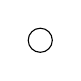
\begin{tikzpicture}[scale=0.051]
					\tikzstyle{every node}+=[inner sep=0pt]
					\draw [black] (29.3,-26.5) circle (3);
				\end{tikzpicture}
			
			\item Transition is denoted by  $\rightarrow$
			
			\item Initial state is denoted by $\rightarrow$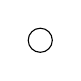
\begin{tikzpicture}[scale=0.051]
				\tikzstyle{every node}+=[inner sep=0pt]
				\draw [black] (29.3,-26.5) circle (3);
			\end{tikzpicture}
			\item Final state is denoted by 
				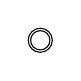
\begin{tikzpicture}[scale=0.051]
					\tikzstyle{every node}+=[inner sep=0pt]
					\draw [black] (49,-17.5) circle (3);
					\draw [black] (49,-17.5) circle (2.4);
				\end{tikzpicture}
			
		\end{itemize}
	\end{itemize}
	
	\begin{center}
	\begin{figure}
			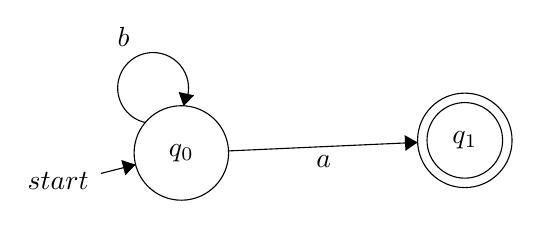
\begin{tikzpicture}[scale=0.2]
			\tikzstyle{every node}+=[inner sep=0pt]
			\draw [black] (22.7,-29.5) circle (3);
			\draw (22.7,-29.5) node {$q_0$};
			\draw [black] (40.7,-28.7) circle (3);
			\draw (40.7,-28.7) node {$q_1$};
			\draw [black] (40.7,-28.7) circle (2.4);
			\draw [black] (17.6,-30.8) -- (19.79,-30.24);
			\draw (16.84,-31.27) node [left] {$start$};
			\fill [black] (19.79,-30.24) -- (18.89,-29.95) -- (19.14,-30.92);
			\draw [black] (25.7,-29.37) -- (37.7,-28.83);
			\fill [black] (37.7,-28.83) -- (36.88,-28.37) -- (36.93,-29.37);
			\draw (31.74,-29.64) node [below] {$a$};
			\draw [black] (20.419,-27.57) arc (257.49857:-30.50143:2.25);
			\draw (19.03,-22.8) node [above] {$b$};
			\fill [black] (22.84,-26.52) -- (23.51,-25.84) -- (22.53,-25.63);
		\end{tikzpicture}
	\caption{Transition digram}
	\end{figure}
	\end{center}
\end{frame}
\begin{frame}{Finite Automata}
	\textbf{Transition Table:}
	\begin{itemize}
		\item A tabular representation in which rows correspond to states, columns 
		correspond to inputs and entries correspond to next states.

		\item The start state is denoted by an arrow with no source.
		\item The accept state is denoted by a star.
	\end{itemize}
\begin{center}
\begin{table}
		\begin{tabular}{ c ||c |c }
		
		State$\setminus$input & a & b \\ 
		\hline
		\hline
		$\rightarrow$q0 & q1 & q0 \\  
		\hline
		*q1 & - & -    \\
		
	\end{tabular}
\caption{Transition Table}
\end{table}
\end{center}
\end{frame}
\begin{frame}{Finite Automata}
	\textbf{There are two types of finite automata}
	\begin{enumerate}
		\item Deterministic Finite Automata (DFA)
 		\item Non-Deterministic Finite Automata (NFA)
	\end{enumerate}
\end{frame}
\section{Deterministic Finite Automata (DFA)}
\begin{frame}{Deterministic Finite Automata (DFA)}
	\textbf{Deterministic Finite Automata (DFA)}
	\begin{itemize}
		\item It is a finite state machine that reads input symbols from an alphabet one by one and transitions between states based on a fixed set of rules.
		\item The transitions are deterministic, meaning that for a given input symbol and current state, there is only one next state. 
		\item DFAs are capable of recognizing and accepting certain types of languages, known as regular languages.
	\end{itemize}
\end{frame}
\begin{frame}{Deterministic Finite Automata (DFA)}
	\textbf{Deterministic Finite Automata (DFA)}
	\begin{itemize}
		\item Formally, a deterministic finite automaton can be represented by a 5-tuple $$M=(Q,\Sigma,\delta,q_0,F)$$
		\begin{itemize}
			\item Q is a finite set of states
			\item $\Sigma$ is a finite input alphabet
			\item $\delta$ is the transition function mapping $ Q \times \Sigma\  to\  Q$ i.e.,$\delta(q,a)$ is a state for each state q and input symbol a.
			\item $q_0 \in Q$ is the initial state
			\item F $\subseteq$ Q is the set of final states.It is assumed here that there may be
			more than one final state.
		\end{itemize}
	\end{itemize}
\end{frame}
\begin{frame}{Deterministic Finite Automata (DFA)}
	\textbf{Steps to design a DFA}
	\begin{enumerate}
		\item Understand the language for which the DFA has to be designed and write 
		the language for the set of strings starting with minimum string that are 
		accepted by FA.

		\item Draw transition diagram for the minimum length string.
		\item Obtain the possible transitions to be made for each state on each input 
		symbol.
		\item Draw the transition table.
		\item Test DFA with few strings that are accepted and few strings that are 
		rejected by the given language.
		\item Represent DFA with tuples.
	\end{enumerate}
\end{frame}
\begin{frame}{Deterministic Finite Automata (DFA)}
	\textbf{Q:}Design DFA that accepts all strings which starts with ‘1’ over the 
	alphabet \{0,1\}
	\begin{itemize}

		\item[1] Understand the language for which the DFA has to be designed and write 
		the language for the set of strings starting with minimum string that are 
		accepted by FA.

		
		$$L = \{1, 10, 11, 100, 110, 101, 111, ................\}$$
		\item[2] Draw transition diagram for the minimum length string.
		\begin{center}
			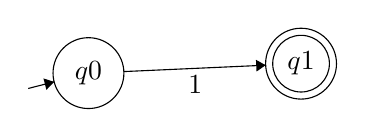
\begin{tikzpicture}[scale=0.15]
				\tikzstyle{every node}+=[inner sep=0pt]
				\draw [black] (22.7,-29.5) circle (3);
				\draw (22.7,-29.5) node {$q0$};
				\draw [black] (40.7,-28.7) circle (3);
				\draw (40.7,-28.7) node {$q1$};
				\draw [black] (40.7,-28.7) circle (2.4);
				\draw [black] (17.6,-30.8) -- (19.79,-30.24);
				\fill [black] (19.79,-30.24) -- (18.89,-29.95) -- (19.14,-30.92);
				\draw [black] (25.7,-29.37) -- (37.7,-28.83);
				\fill [black] (37.7,-28.83) -- (36.88,-28.37) -- (36.93,-29.37);
				\draw (31.74,-29.64) node [below] {$1$};
			\end{tikzpicture}
		\end{center}
\end{itemize}
\end{frame}
\begin{frame}{Deterministic Finite Automata (DFA)}

		\begin{itemize}
			 \item[3] Obtain the possible transitions to be made for each state on each input 
			symbol.
			\begin{center}
				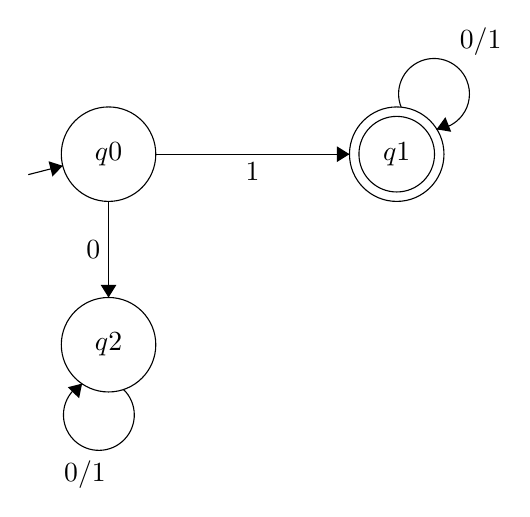
\begin{tikzpicture}[scale=0.2]
					\tikzstyle{every node}+=[inner sep=0pt]
					\draw [black] (22.4,-28.7) circle (3);
					\draw (22.4,-28.7) node {$q0$};
					\draw [black] (40.7,-28.7) circle (3);
					\draw (40.7,-28.7) node {$q1$};
					\draw [black] (40.7,-28.7) circle (2.4);
					\draw [black] (22.4,-40.8) circle (3);
					\draw (22.4,-40.8) node {$q2$};
					\draw [black] (17.3,-30) -- (19.49,-29.44);
					\fill [black] (19.49,-29.44) -- (18.59,-29.15) -- (18.84,-30.12);
					\draw [black] (25.4,-28.7) -- (37.7,-28.7);
					\fill [black] (37.7,-28.7) -- (36.9,-28.2) -- (36.9,-29.2);
					\draw (31.55,-29.2) node [below] {$1$};
					\draw [black] (40.986,-25.725) arc (202.24052:-85.75948:2.25);
					\draw (46.03,-22.46) node [above] {$0/1$};
					\fill [black] (43.23,-27.12) -- (44.16,-27.28) -- (43.79,-26.35);
					\draw [black] (22.4,-31.7) -- (22.4,-37.8);
					\fill [black] (22.4,-37.8) -- (22.9,-37) -- (21.9,-37);
					\draw (21.9,-34.75) node [left] {$0$};
					\draw [black] (23.344,-43.635) arc (46.14669:-241.85331:2.25);
					\draw (20.9,-48.15) node [below] {$0/1$};
					\fill [black] (20.72,-43.27) -- (19.81,-43.5) -- (20.53,-44.2);
				\end{tikzpicture}
			\end{center}			
		\end{itemize}
\end{frame}
\begin{frame}{Deterministic Finite Automata (DFA)}
	
	\begin{itemize}
		\item[4] Draw the transition table.
		\begin{center}
				\begin{tabular}{ c ||c |c }
				
				& 0 & 1 \\ 
				\hline 
				\hline
				$\rightarrow$q0 & q2 & q1 \\  
				\hline
				*q1 & q1 & q1    \\
					\hline
				q2 & q2 & q2    \\
			\end{tabular}
		\end{center}
		\item Test DFA with few strings that are accepted and few strings that are 
		rejected by the given language.
		\item Represent DFA with tuples.
		
	\end{itemize}
\end{frame}
\begin{frame}{Deterministic Finite Automata (DFA)}
	
	\begin{itemize}
		\item[5] Test DFA with few strings that are accepted and few strings that are 
		rejected by the given language.
		\begin{itemize}
			\item \textbf{Case i)} Let w=1010 $\in$ L
		\begin{center}
				\begin{tabular}{c c c}
				$\delta$(q0,1010) & = & $\delta$(q1,010) \\
				& = & $\delta$(q1,10) \\
				&=& $\delta$(q1,0) \\
				& = & q1
			\end{tabular}
		\end{center}
		
			q1 is final state and the entire string has been consumed i.e., given string 
			is accepted by DFA.
			
			\item \textbf{Case ii)} Let w=0001 $\notin$ L
				\begin{center}
				\begin{tabular}{c c c}
		$\delta$(q0,0001) &=&$\delta$(q2,001)\\ 
			&=& $\delta$(q2,01)\\
			&=& $\delta$(q2,1)\\
			&=& q2\\
				\end{tabular}
		\end{center}
			q2 is not final state and the entire string has been consumed i.e., given 
			string is rejected by DFA
		\end{itemize}
		
		\item Represent DFA with tuples.
		
	\end{itemize}
\end{frame}
\begin{frame}{Deterministic Finite Automata (DFA)}
	
	\begin{itemize}	
		\item[6] Represent DFA with tuples.
		$$	DFA, M = (Q,\Sigma,\delta,q_0,F)$$
		\begin{eqnarray*}
		where\  Q &=& \{q0, q1, q2\} \\
		\Sigma &=& \{ 0,1 \} \\
		\delta: \delta(q0,0)&=&q2 \\
		\delta(q0,1)&=&q1 \\
		\delta(q1,0)&=&q1 \\
	\delta(q1,1)&=&q1
 \\
	\delta(q2,0)&=&q2 \\
	\delta(q2,1)&=&q2 \\
		q0 – initial\  state& = & q0\\
			F – final state & =& \{ q1\}
		\end{eqnarray*}
	\end{itemize}
\end{frame}
\begin{frame}{Deterministic Finite Automata (DFA)}
\textbf{Dead State:}  A rejecting state that is essentially a dead end. Once the machine enters a dead state, there is no way for it to reach an accepting state, so we already know that the string is going to be rejected.
	\begin{center}
	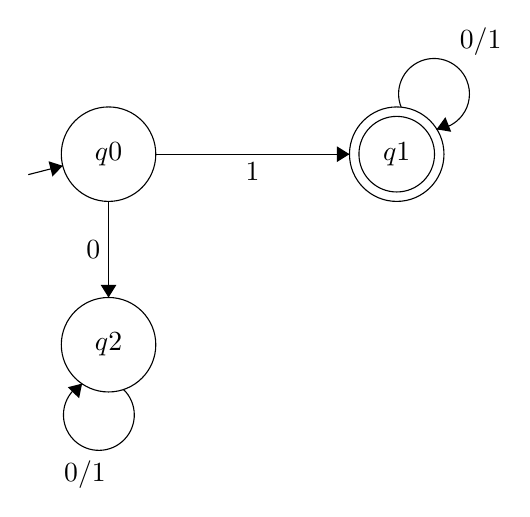
\begin{tikzpicture}[scale=0.2]
		\tikzstyle{every node}+=[inner sep=0pt]
		\draw [black] (22.4,-28.7) circle (3);
		\draw (22.4,-28.7) node {$q0$};
		\draw [black] (40.7,-28.7) circle (3);
		\draw (40.7,-28.7) node {$q1$};
		\draw [black] (40.7,-28.7) circle (2.4);
		\draw [black] (22.4,-40.8) circle (3);
		\draw (22.4,-40.8) node {$q2$};
		\draw [black] (17.3,-30) -- (19.49,-29.44);
		\fill [black] (19.49,-29.44) -- (18.59,-29.15) -- (18.84,-30.12);
		\draw [black] (25.4,-28.7) -- (37.7,-28.7);
		\fill [black] (37.7,-28.7) -- (36.9,-28.2) -- (36.9,-29.2);
		\draw (31.55,-29.2) node [below] {$1$};
		\draw [black] (40.986,-25.725) arc (202.24052:-85.75948:2.25);
		\draw (46.03,-22.46) node [above] {$0/1$};
		\fill [black] (43.23,-27.12) -- (44.16,-27.28) -- (43.79,-26.35);
		\draw [black] (22.4,-31.7) -- (22.4,-37.8);
		\fill [black] (22.4,-37.8) -- (22.9,-37) -- (21.9,-37);
		\draw (21.9,-34.75) node [left] {$0$};
		\draw [black] (23.344,-43.635) arc (46.14669:-241.85331:2.25);
		\draw (20.9,-48.15) node [below] {$0/1$};
		\fill [black] (20.72,-43.27) -- (19.81,-43.5) -- (20.53,-44.2);
	\end{tikzpicture}
state $q_2$ is a dead state
\end{center}			
\end{frame}
\begin{frame}{Deterministic Finite Automata (DFA)}
	\textbf{Language acceptd by a DFA}
	\begin{itemize}
		\item The language accepted by a DFA M is the set of all string accepted by M .
		\item It is denoted by $L(M).$
		$$L(M)=\{w\in\Sigma^*/M \ accepts \ w\}$$
	\end{itemize}
\end{frame}
\begin{frame}{Deterministic Finite Automata (DFA)}
	\textbf{Extending the transition function to string\\ (Extended transition function - $\hat{\delta}$)}
	\begin{itemize}
		\item It is a function that takes a state q and a string w and return a state p.
		\item \textbf{Example:}
		\begin{itemize}
			\item consider a string w =101
			\item generally we write the transition function as 
			$$\delta(\delta(\delta(q0,1),0),1)$$
			\item Instead of that we can write.
			$$\hat{\delta}(q0,101)$$
			\item generally $\hat{\delta}(q0,w)=p$
			\item if p$\in$f then w is accepted
		\end{itemize}
	\end{itemize}
\end{frame}
\begin{frame}{Deterministic Finite Automata (DFA)}
	\textbf{ Properties of $\hat{\delta}$}
	\begin{enumerate}
		\item $\hat{\delta}(qo,\epsilon)=q0$
		\item $\hat{\delta}(qo,wa)=\delta(\hat{\delta}(q0,w),a)$
		$$\delta: Q \times \Sigma\rightarrow Q$$
		$$\hat{\delta}: Q \times \Sigma^*\rightarrow Q$$
		\item $\hat{\delta}=\delta$
		\begin{eqnarray*}
			\hat{\delta}(q,a)&=&\hat{\delta}(q,\epsilon a)\\
		&=&\delta(\hat{\delta}(q,\epsilon),a)\\
			&=&\delta(q,a)\\
			\hat{\delta}&=&\delta
		\end{eqnarray*}
	\end{enumerate}
\end{frame}
\begin{frame}{Deterministic Finite Automata (DFA)}
	\textbf{Language acceptd by a DFA}
	\begin{itemize}
		\item Set of all string accepted by the finite automata.
		\item It is denoted by $L(M).$
		$$L(M)=\{w/\hat{\delta}(q_0,w)=p  \ and \ p \in f\}$$
	\end{itemize}
\end{frame}
\section{Nondeterministic finite automaton (NFA)}
\begin{frame}{Nondeterministic finite automaton (NFA)}
	Nondeterminisim means a choice of moves for an automaton. Rather than prescribing a unique move in each situation
	\par The transition function that a state \& input symbol as arguments , but returns a set of zero , one or more states.\\
	
\end{frame}
\begin{frame}{Nondeterministic finite automaton (NFA)}
	\textbf{Nondeterministic finite automaton (NFA)}
	\begin{itemize}
		\item Formally, a Nondeterministic finite automaton can be represented by a 5-tuple $$M=(Q,\Sigma,\delta,q_0,f)$$
		\begin{itemize}
			\item Q is a finite set of states
			\item $\Sigma$ is a finite input alphabet
			\item $\delta$ is the transition function mapping $ Q \times \Sigma\  into\  2^Q$, (which is the 
			power set of Q, the set of all subsets of Q;)
			\item $q_0 \in Q$ is the initial state
			\item F $\subseteq$ Q is the set of final states.(It is assumed here that there may be
			more than one final state.)
		\end{itemize}
	\end{itemize}
\end{frame}
\begin{frame}{Nondeterministic finite automaton (NFA)}
	\textbf{Example:}\\
	NFA that accepts strings which contains either two 
	consecutive 0’s or two consecutive 1’s.
	$$L=\{00,11,100,001,110,011,111,000,0100,1011,........\}$$
	\begin{figure}
	
		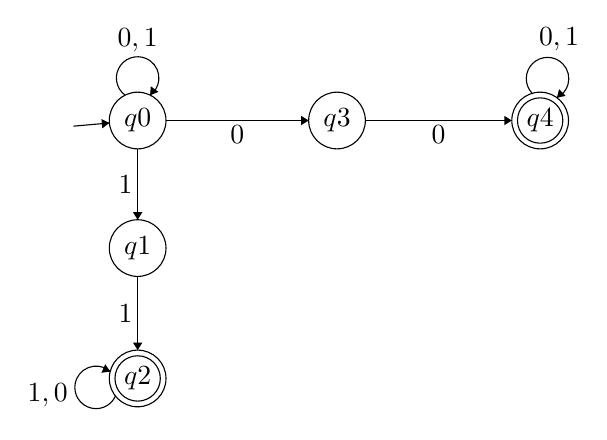
\begin{tikzpicture}[scale=0.12]
			\tikzstyle{every node}+=[inner sep=0pt]
			\draw [black] (41.5,-16.6) circle (3);
			\draw (41.5,-16.6) node {$q3$};
			\draw [black] (63,-16.6) circle (3);
			\draw (63,-16.6) node {$q4$};
			\draw [black] (63,-16.6) circle (2.4);
			\draw [black] (20.4,-30.1) circle (3);
			\draw (20.4,-30.1) node {$q1$};
			\draw [black] (20.4,-43.9) circle (3);
			\draw (20.4,-43.9) node {$q2$};
			\draw [black] (20.4,-43.9) circle (2.4);
			\draw [black] (20.4,-16.6) circle (3);
			\draw (20.4,-16.6) node {$q0$};
			\draw [black] (44.5,-16.6) -- (60,-16.6);
			\fill [black] (60,-16.6) -- (59.2,-16.1) -- (59.2,-17.1);
			\draw (52.25,-17.1) node [below] {$0$};
			\draw [black] (62.163,-13.731) arc (223.99202:-64.00798:2.25);
			\draw (65,-9.29) node [above] {$0,1$};
			\fill [black] (64.77,-14.19) -- (65.69,-13.99) -- (65,-13.28);
			\draw [black] (20.4,-33.1) -- (20.4,-40.9);
			\fill [black] (20.4,-40.9) -- (20.9,-40.1) -- (19.9,-40.1);
			\draw (19.9,-37) node [left] {$1$};
			\draw [black] (18.057,-45.755) arc (-23.90524:-311.90524:2.25);
			\draw (13.05,-45.67) node [left] {$1,0$};
			\fill [black] (17.5,-43.17) -- (16.97,-42.39) -- (16.57,-43.3);
			\draw [black] (19.077,-13.92) arc (234:-54:2.25);
			\draw (20.4,-9.35) node [above] {$0,1$};
			\fill [black] (21.72,-13.92) -- (22.6,-13.57) -- (21.79,-12.98);
			\draw [black] (13.6,-17.2) -- (17.41,-16.86);
			\fill [black] (17.41,-16.86) -- (16.57,-16.44) -- (16.66,-17.43);
			\draw [black] (20.4,-19.6) -- (20.4,-27.1);
			\fill [black] (20.4,-27.1) -- (20.9,-26.3) -- (19.9,-26.3);
			\draw (19.9,-23.35) node [left] {$1$};
			\draw [black] (23.4,-16.6) -- (38.5,-16.6);
			\fill [black] (38.5,-16.6) -- (37.7,-16.1) -- (37.7,-17.1);
			\draw (30.95,-17.1) node [below] {$0$};
		\end{tikzpicture}
	
	\caption{Transition Diagram}
	\end{figure}
\end{frame}
\begin{frame}{Nondeterministic finite automaton (NFA)}
	\textbf{Example Cont..}\\
	\begin{center}
		\begin{table}
			\begin{tabular}{ c ||c |c }
				
				State$\setminus$input & 0 & 1 \\ 
				\hline
				\hline
				$\rightarrow$q0 & \{q0,q3\} & \{q0,q1\} \\  
				\hline
				q1 & $\phi$& \{q2\}    \\
					\hline
				*q2 & \{q2\} & \{q2\}    \\
					\hline
				q3 & \{q4\} & $\phi$    \\
					\hline
				*q4 & \{q4\} & \{q4\}   \\				
			\end{tabular}
			\caption{Transition Table}
		\end{table}
	\end{center}
\end{frame}
\begin{frame}{Nondeterministic finite automaton (NFA)}
	\textbf{Example Cont..}\\
	Let the input, $w = 01001 \in L$
	\begin{eqnarray*}
		\delta(q0,0)&=&\{q0,q3\}\\
		\hat{\delta}(q0,01)&=&\delta(\delta(q0,0),1)\\
						&=&\delta(\{q0,q3\},1)\\
						&=&\delta(q0,1)\cup \delta(q3,1)\\
						&=&\{q0,q1\} \cup \phi\\
						&=&\{q0,q1\}\\
		\hat{\delta}(q0,010)&=&\delta(\hat{\delta}(q0,01),0)\\
						&=&\delta(\{q0,q1\},0)\\
						&=&\delta(qo,0) \cup \delta(q1,0)\\
						&=&\{qo,q3\}\cup \phi\\
						&=&\{q0,q3\}\\
	%	\hat{\delta}(q0,0100)&=&\delta(\hat{\delta}(q0,010),0)\\
	\end{eqnarray*}
\end{frame}
\begin{frame}{Nondeterministic finite automaton (NFA)}
	\textbf{Example Cont..}\\
	\begin{eqnarray*}
			\hat{\delta}(q0,0100)&=&\delta(\hat{\delta}(q0,010),0)\\
								&=&\delta(\{q0,q3\},0)\\
								&=&\delta(q0,0)\cup \delta(q3,0)\\
								&=&\{q0,q3\}\cup \{q4\}\\
								&=&\{q0,q3,q4\}\\
			\hat{\delta}(q0,01001)&=&\delta(\hat{\delta}(q0,0100),1)\\
								&=&\delta(\{q0,q3,q4\},1)\\
								&=&\delta(qo,1)\cup\delta(q3,1)\cup\delta(q4,1)\\
								&=&\{q0,q1\}\cup\phi \cup \{q4\}\\
								&=&\{q0,q1,q4\}
	\end{eqnarray*}
After the entire string is consumed, the FA is in the state q4.
As q4 is the final state, the string is a accepted by FA
\end{frame}
\begin{frame}{Nondeterministic finite automaton (NFA)}
	\textbf{Example Cont..}\\
	$	M=(Q,\Sigma,\delta,q_0,F)$
	\tiny
	\begin{eqnarray*}
		where \  Q &=& \{q0, q1, q2, q3,q4\}\\
		\Sigma &=&  \{ 0,1 \}\\
		\delta:\delta(q0,0)&=&\{q0,q3\}\\
		\delta(q0,1)&=&\{q0,q1\}\\
		\delta(q1,0)&=&\phi\\
		\delta(q1,1)&=&\{q2\}\\
		\delta(q2,0)&=&\{q2\}\\
		\delta(q2,1)&=&\{q2\}\\
		\delta(q3,0)&=&\{q4\}\\
		\delta(q3,1)&=&\phi\\
		\delta(q4,0)&=&\{q4\}\\
		\delta(q4,1)&=&\{q4\}\\
		q_0 &=& q0\\
		F &=& \{ q2,q4\}
	\end{eqnarray*}
\end{frame}
\begin{frame}{Nondeterministic finite automaton (NFA)}
	\textbf{The extended transition function}
	\begin{enumerate}
		\item $\hat{\delta}$(q,$\epsilon$)=q
		\begin{itemize}
			\item NFA cannot change its state without accepting an input symbol
		\end{itemize}
	\item $\hat{\delta}(q,wa)=\{p/ \ for\  some\  state\ r \ in \ \hat{\delta}(q,w), for\  some\  state\  p\  \ in \ \delta(r,a)\}$
	\begin{itemize}
		\item $\hat{\delta}(q,w)=\{r1,r2,r3,r4,.....\}$
		\item $\delta(\hat{\delta}(q,w),a)=\delta(\{r1,r2,r3,r4,.....\},a)=\{p1,p2,p3,p4,....\}$
	\end{itemize}
\item $\hat{\delta}(q,a)$=$\delta(q,a)$
\begin{itemize}
	\item $\hat{\delta}(q,a)=\hat{\delta}(q,\epsilon a)=\delta(\hat{\delta}(q,\epsilon),a)=\delta(q,a)$
	\item $\hat{\delta}$=$\delta$
\end{itemize}
\item $\delta(p,w)=\bigcup\limits_{q\ in \ p}\delta(q,w)$
\begin{itemize}
	\item Suppose p=\{q1,q2,q3,...,qn\}
\end{itemize}
	\end{enumerate}
\small
\begin{eqnarray*}
	\delta(\{q1,q2,q3,...,qn\},w)&=&\delta(q1,w)\cup\delta(q2,w)\cup....\delta(qn,w)\\
								&=&\bigcup\limits_{i=1}^{n}\delta(q_i,w)
\end{eqnarray*}

\end{frame}
\begin{frame}{Nondeterministic finite automaton (NFA)}
	\textbf{The Language accepted by an NFA}
	\begin{itemize}
		\item Set of all string accepted by an NFA is called language accepted by an NFA
	\end{itemize}
\begin{eqnarray*}
	L(M)&=&\{x/\hat{\delta}(q,x) \ is \ in \ f\}\\
	&or&\\
	  L(M)&=&\{w/\hat{\delta}(q0,w)\cap f\neq \phi\}
\end{eqnarray*}
$\hat{\delta}(q,w)$ contain a final state then it is accepted
	\begin{center}
		\textbf{All DFA's are NFA's}
	\end{center}
\end{frame}
\begin{frame}{Differences between NFA and DFA}
\begin{center}
	\begin{table}
		\begin{tabular}{|p{5.5cm}|p{5.5cm}|}
			\hline
			\centering	\textbf{NFA} & 	\textbf{DFA}\\
			\hline
			A Nondeterministic finite automaton is a 5-tuple $M=(Q,\Sigma,\delta,q_0,f)$  where $\delta: Q\times \Sigma \ into \ 2^Q$ & A Deterministic finite 
			automaton is a 5-tuple $M=(Q,\Sigma,\delta,q_0,f)$  where $\delta: Q\times \Sigma \ into \ Q$ \\
			\hline
			NFA is the one in which there 
			exists many paths for a specific 
			input from current state to next 
			state.
 & DFA is a FA in which there is only 
			one path for a specific input from 
			current state to next state.\\
			\hline
			Next move cannot be determind by the present state and current input symbol. & Next move can be determind by the present state and current input symbol.\\
			\hline
			NFA is easier to construct. & DFA is more difficult to construct.\\
			\hline
			NFA requires less space. & dfa requires more space.\\
			\hline
			Time required for executing an 
			input string is more. & Time required for executing an 
			input string is less\\
			\hline
		\end{tabular}
	\caption{Differences between NFA and DFA}
	\end{table}
\end{center}
\end{frame}
\begin{frame}{Finite Automata}
	\textbf{Applications of FA:}
\begin{itemize}
	\item Used in Lexical analysis phase of a compiler to recognize tokens.
	\item Used in text editors for string matching.
	\item Software for designing and checking the behavior of digital circuits.
\end{itemize}
		\textbf{Limitations of FA:}
		\begin{itemize}
\item FA’s will have finite amount of memory.
\item The class of languages recognized by FA s is strictly the regular set. 
	There are certain languages which are non regular i.e. cannot be 
	recognized by any FA.

\end{itemize}
\end{frame}

\begin{frame}{Finite Automata}
	\textbf{NFA to DFA Conversion}\\
	Let, $M = (Q, \Sigma, \delta, q0, F)$ is an NFA which accepts the language L(M). There should be equivalent DFA denoted by $M' = (Q', \Sigma', q0', \delta', F')$ such that$ L(M) = L(M')$.
\begin{enumerate}
	\item Initially Q' = $\phi$
	\item Add q0 of NFA to Q'. Then find the transitions from this start state.
	\item In Q', find the possible set of states for each input symbol. If this set of states is not in Q', then add it to Q'.
	\item In DFA, the final state will be all the states which contain F(final states of NFA)
\end{enumerate}
\end{frame}
\begin{frame}{Finite Automata}
	\textbf{Q:}Convert the given NFA to DFA.
	\begin{figure}
		\begin{center}
			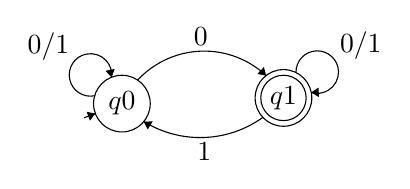
\begin{tikzpicture}[scale=0.12]
				\tikzstyle{every node}+=[inner sep=0pt]
				\draw [black] (16.2,-28.9) circle (3);
				\draw (16.2,-28.9) node {$q0$};
				\draw [black] (33.3,-28.3) circle (3);
				\draw (33.3,-28.3) node {$q1$};
				\draw [black] (33.3,-28.3) circle (2.4);
				\draw [black] (17.863,-26.418) arc (137.21873:46.80037:9.591);
				\fill [black] (31.47,-25.94) -- (31.23,-25.03) -- (30.54,-25.76);
				\draw (24.54,-22.81) node [above] {$0$};
				\draw [black] (13.329,-28.069) arc (281.59201:-6.40799:2.25);
				\draw (10.68,-22.89) node [left] {$0/1$};
				\fill [black] (15.11,-26.12) -- (15.44,-25.23) -- (14.46,-25.43);
				\draw [black] (31.125,-30.353) arc (-54.22794:-121.75295:11.352);
				\fill [black] (18.51,-30.8) -- (18.93,-31.64) -- (19.46,-30.79);
				\draw (24.91,-33.02) node [below] {$1$};
				\draw [black] (34.625,-25.622) arc (181.40536:-106.59464:2.25);
				\draw (39.23,-22.79) node [right] {$0/1$};
				\fill [black] (36.23,-27.72) -- (37.04,-28.2) -- (37.02,-27.2);
				\draw [black] (12.2,-30.4) -- (13.39,-29.95);
				\fill [black] (13.39,-29.95) -- (12.47,-29.77) -- (12.82,-30.7);
			\end{tikzpicture}
		\end{center}
	\caption{NFA}
	\end{figure}
\textbf{Solution:} For the given transition diagram we will first construct the transition table.
\begin{table}
	\begin{tabular}{c||c|c}
		$\delta$&0&1\\
		\hline
		\hline
		$\rightarrow$q0	&\{q0, q1\}&\{q0\}\\
		*q1&\{q1\}&\{q0, q1\}\\
	\end{tabular}
\end{table}
\end{frame}
\begin{frame}{Convert the given NFA to DFA}
Now we will obtain $\delta$' transition for state q0.
\begin{eqnarray*}
	\delta'([q0], 0) &=& \{q0, q1\}  \\
	&=& [q0, q1]      \ \  \textbf{(new state generated)  }\\
	\delta'([q0], 1) &=& \{q1\} = [q1]  
\end{eqnarray*}
The $\delta$' transition for state q1 is obtained as:
\begin{eqnarray*}
\delta'([q1], 0) &=& \{q1\} \\ 
\delta'([q1], 1) &=& \{q0, q1\}  
\end{eqnarray*}
Now we will obtain $\delta$' transition on [q0, q1].
\begin{eqnarray*}
	\delta'([q0, q1], 0) &=& \delta(q0, 0) \cup \delta(q1, 0)  \\
	&=& \{q0, q1\} \cup \{q1\}\\  
	&=& \{q0, q1\}\\  
	&=& [q0, q1]\\  
\end{eqnarray*}
\end{frame}
\begin{frame}{Convert the given NFA to DFA}
Similarly
\begin{eqnarray*}
	\delta'([q0, q1], 1) &=& \delta(q0, 1) \cup \delta(q1, 1)  \\
	&=& \{q0\} \cup \{q0, q1\}  \\
	&=& \{q0, q1\}  \\
	&=& [q0, q1]  
\end{eqnarray*}
As in the given NFA, q1 is a final state, then in DFA wherever, q1 exists that state becomes a final state. Hence in the DFA, final states are [q1] and [q0, q1].\\
The transition table for the constructed DFA will be:
\begin{table}
	\begin{tabular}{c||c|c}
		$\delta$&0&1\\
		\hline
		\hline
		$\rightarrow$[q0]&[q0, q1]&[q0]\\
			\hline
		*[q1]&[q1]&[q0, q1]\\
			\hline
		*[q0, q1]&[q0, q1]&[q0, q1]
	\end{tabular}
\caption{Transition table}
\end{table}
\end{frame}
\begin{frame}{Convert the given NFA to DFA}
The Transition diagram will be:
\begin{figure}
	\begin{center}
	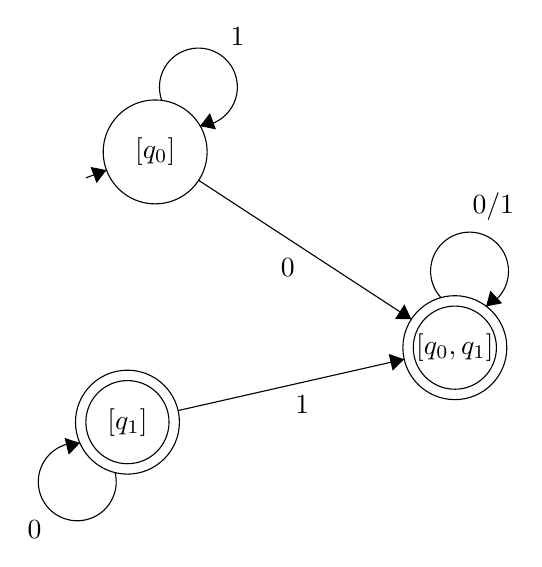
\begin{tikzpicture}[scale=0.22]
		\tikzstyle{every node}+=[inner sep=0pt]
		\draw [black] (14.3,-22.5) circle (3);
		\draw (14.3,-22.5) node {$[q_0]$};
		\draw [black] (12.7,-38.1) circle (3);
		\draw (12.7,-38.1) node {$[q_1]$};
		\draw [black] (12.7,-38.1) circle (2.4);
		\draw [black] (31.6,-33.8) circle (3);
		\draw (31.6,-33.8) node {$[q_0,q_1]$};
		\draw [black] (31.6,-33.8) circle (2.4);
		\draw [black] (11.986,-41.002) arc (13.91676:-274.08324:2.25);
		\draw (7.34,-43.76) node [below] {$0$};
		\fill [black] (9.96,-39.3) -- (9.07,-39.01) -- (9.31,-39.98);
		\draw [black] (10.3,-24) -- (11.49,-23.55);
		\fill [black] (11.49,-23.55) -- (10.57,-23.37) -- (10.92,-24.3);
		\draw [black] (16.81,-24.14) -- (29.09,-32.16);
		\fill [black] (29.09,-32.16) -- (28.69,-31.3) -- (28.15,-32.14);
		\draw (21.95,-28.65) node [below] {$0$};
		\draw [black] (15.63,-37.43) -- (28.67,-34.47);
		\fill [black] (28.67,-34.47) -- (27.78,-34.16) -- (28.01,-35.13);
		\draw (22.8,-36.53) node [below] {$1$};
		\draw [black] (30.807,-30.919) arc (223.11447:-64.88553:2.25);
		\draw (33.82,-26.51) node [above] {$0/1$};
		\fill [black] (33.4,-31.42) -- (34.33,-31.24) -- (33.65,-30.51);
		\draw [black] (14.687,-19.537) arc (200.28531:-87.71469:2.25);
		\draw (19.05,-16.39) node [above] {$1$};
		\fill [black] (16.89,-21.01) -- (17.81,-21.2) -- (17.46,-20.26);
	\end{tikzpicture}
	\end{center}
\caption{Transition Digram - DFA}
\end{figure}
\end{frame}
\begin{frame}{Convert the given NFA to DFA}
	Even we can change the name of the states of DFA.
	\begin{eqnarray*}
		A &=& [q0]  \\
		B &=& [q1]  \\
		C &=& [q0, q1] 
	\end{eqnarray*}
\begin{figure}
	\begin{center}
	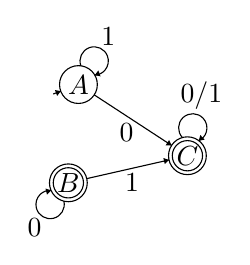
\begin{tikzpicture}[scale=0.08]
			\tikzstyle{every node}+=[inner sep=0pt]
			\draw [black] (14.3,-22.5) circle (3);
			\draw (14.3,-22.5) node {$A$};
			\draw [black] (12.7,-38.1) circle (3);
			\draw (12.7,-38.1) node {$B$};
			\draw [black] (12.7,-38.1) circle (2.4);
			\draw [black] (31.6,-33.8) circle (3);
			\draw (31.6,-33.8) node {$C$};
			\draw [black] (31.6,-33.8) circle (2.4);
			\draw [black] (11.986,-41.002) arc (13.91676:-274.08324:2.25);
			\draw (7.34,-43.76) node [below] {$0$};
			\fill [black] (9.96,-39.3) -- (9.07,-39.01) -- (9.31,-39.98);
			\draw [black] (10.3,-24) -- (11.49,-23.55);
			\fill [black] (11.49,-23.55) -- (10.57,-23.37) -- (10.92,-24.3);
			\draw [black] (16.81,-24.14) -- (29.09,-32.16);
			\fill [black] (29.09,-32.16) -- (28.69,-31.3) -- (28.15,-32.14);
			\draw (21.95,-28.65) node [below] {$0$};
			\draw [black] (15.63,-37.43) -- (28.67,-34.47);
			\fill [black] (28.67,-34.47) -- (27.78,-34.16) -- (28.01,-35.13);
			\draw (22.8,-36.53) node [below] {$1$};
			\draw [black] (30.807,-30.919) arc (223.11447:-64.88553:2.25);
			\draw (33.82,-26.51) node [above] {$0/1$};
			\fill [black] (33.4,-31.42) -- (34.33,-31.24) -- (33.65,-30.51);
			\draw [black] (14.687,-19.537) arc (200.28531:-87.71469:2.25);
			\draw (19.05,-16.39) node [above] {$1$};
			\fill [black] (16.89,-21.01) -- (17.81,-21.2) -- (17.46,-20.26);
	\end{tikzpicture}
	\end{center}
\caption{Transition diagram -DFA}
\end{figure}
Upon careful inspection, it appears that state $B$ is unreachable from the initial state $A$. Thus, for the purpose of minimizing the DFA, it is advisable to remove state $B$.
\end{frame}
\begin{frame}{Equivalence of NFA and DFA}
\textbf{Equivalence of NFA and DFA}
\begin{itemize}
	\item If L is a Language accepted by an NFA then there is a DFA that accept L
	\begin{itemize}
		\item i.e for every NFA there exist an equivalent DFA
		\item The transition of NFA to DFA is normally called a subset construction
	\end{itemize}
\end{itemize}
\end{frame}
\begin{frame}{Equivalence of NFA and DFA}
	\begin{block}{Theorem 1.0}
		Let language $L \subseteq \Sigma^*$, and suppose L is accepted by NFA $N = (\Sigma, Q, q0, F, \delta)$. There exists a DFA $D= (\Sigma, Q’, q0', F’, \delta’)$ that also accepts L. $(L(N) = L(D))$.
	\end{block}
By allowing each state in the DFA D to represent a set of states in the NFA N, we are able to prove through induction that D is equivalent to N. Before we begin the proof, let’s define the parameters of D:
\begin{itemize}
	\item Q’ is equal to the powerset of Q, $Q’ = 2^Q$
	\item $q_0' = \{q_0\}$
	\item F’ is the set of states in Q’ that contain any element of F, $F’ = \{q \in Q’/q \cap F \neq \phi\}$
	\item $\delta$’ is the transition function for D.  $\delta{'}(q, a) = \bigcup_{p \in q} \delta(p, a)\  for\  q \in Q’\  and \ a\in \Sigma.$
\end{itemize}
\end{frame}
\begin{frame}{Equivalence of NFA and DFA}
Now we will prove that $\hat\delta'(q_0,x) = \hat\delta(q_0, x)$ for every x. ie, L(D) = L(N)\\
\textbf{Basis Step:}
	\begin{itemize}
		\item Let x be the empty string $\epsilon$.
		\item By the definition of extended transition function, NFA \& DFA cannot change its state without accepting an input symbol
	\end{itemize}
\begin{eqnarray*}
\hat{\delta'}(q_0,\epsilon) &=& \{q_0\}\\
	\hat{\delta}(q_0,\epsilon) &=& \{q_0\}\\
\end{eqnarray*}
Therefor $\delta'(q_0,\epsilon)=\delta(q_0,\epsilon)$ is true for $x=\epsilon$. \\
\textbf{Inductive Step:}
\begin{itemize}
	\item Assume that for any $y$ with $|y| \geq 0, \hat\delta'(q_0,y) = \hat\delta(q_0, y)$.
	\begin{itemize}
		\item Let both state be $p=\{p_1,p_2,p_3...\}$
	\end{itemize}
	\item Let $n = |y|$, then we need to prove that for a string z with $|z| = n + 1, \hat\delta'(q_0,z) = \hat\delta(q_0, z)$. 
\end{itemize}
\end{frame}

\begin{frame}{Equivalence of NFA and DFA}
\begin{itemize}
	
	\item We can represent the string $z$ as a concatenation of string y $(|y| = n)$ and symbol $a$ from the alphabet $\Sigma. (a \in \Sigma).$ So, $z = ya$.
	\small
	\begin{eqnarray*}
		 \hat\delta'(q_0,z) &=& \hat\delta'(q_0, ya)\\
		 					&=& \delta'(\hat\delta'(q_0, y),a)\\
		 					&=& \delta'(\hat\delta(q_0, y),a)  \ \ (by \ assumption)\\
		 					&=& \bigcup\limits_{p\in\hat{\delta}(q_0,y)}\delta'(p,a)\ \  \  (by\ definition \ of \  \hat{\delta}) \\
		 					&=& \bigcup\limits_{p\in\hat{\delta}(q_0,y)}\delta(p,a)\ \  \  (by \ assumption) \\
		 					&=&\hat{\delta}(q_0,ya) \\
		 					&=&\hat{\delta}(q_0,z)\\
	\end{eqnarray*}
	\item DFA $D$ accepts $a$ string $x$ iff $\hat\delta'(q_0, x) \in F'.$ From the above it follows that D accepts x iff  $\hat\delta(q_0, x) \cap F \neq \phi$.
	\item So a string is accepted by DFA D if, and only if, it is accepted by NFA N.
\end{itemize}
\end{frame}

\subsection{NFA with $\epsilon$ transitions ($\epsilon$-NFA)}

\begin{frame}{NFA with $\epsilon$ transitions($\epsilon$-NFA)}
	In the case of $\epsilon$-NFA without applying an input symbol the state will change
	\\
	\textbf{Formal Definition of NFA with $\epsilon$ transitions}
	$$ 	M=(Q,\Sigma,\delta,q_0,F) $$
	where
	\begin{itemize}
		\item Q is a set of states,
		\item $\Sigma$ is the alphabet, 
		\item $\delta$ is the transition function $\delta: Q\times \{\Sigma \cup \epsilon \} $ into $2^Q$, 
		\item q0 is the initial state,
		\item $F\subset Q$ is the set of final (or accepting) states.
	\end{itemize}
$\delta(q,a)$ will consists of all states p such that there is a transition labelled a from q to p. Where a is either $\epsilon$ or a symbol in $\Sigma$.
\end{frame}
\begin{frame}{NFA with $\epsilon$ transitions($\epsilon$-NFA)}
	\textbf{Example:}
\begin{center}
	\begin{figure}
		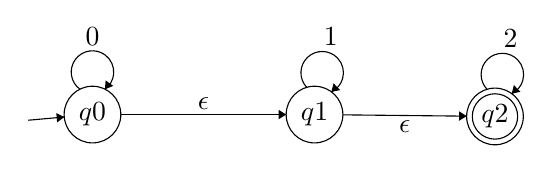
\begin{tikzpicture}[scale=0.12]
			\tikzstyle{every node}+=[inner sep=0pt]
			\draw [black] (63,-16.6) circle (3);
			\draw (63,-16.6) node {$q2$};
			\draw [black] (63,-16.6) circle (2.4);
			\draw [black] (20.4,-16.4) circle (3);
			\draw (20.4,-16.4) node {$q0$};
			\draw [black] (43.9,-16.4) circle (3);
			\draw (43.9,-16.4) node {$q1$};
			\draw [black] (62.163,-13.731) arc (223.99202:-64.00798:2.25);
			\draw (64.65,-9.36) node [above] {$2$};
			\fill [black] (64.77,-14.19) -- (65.69,-13.99) -- (65,-13.28);
			\draw [black] (19.077,-13.72) arc (234:-54:2.25);
			\draw (20.4,-9.15) node [above] {$0$};
			\fill [black] (21.72,-13.72) -- (22.6,-13.37) -- (21.79,-12.78);
			\draw [black] (13.6,-17) -- (17.41,-16.66);
			\fill [black] (17.41,-16.66) -- (16.57,-16.24) -- (16.66,-17.23);
			\draw [black] (43.082,-13.526) arc (223.6158:-64.3842:2.25);
			\draw (45.62,-9.17) node [above] {$1$};
			\fill [black] (45.68,-14) -- (46.61,-13.81) -- (45.92,-13.09);
			\draw [black] (23.4,-16.4) -- (40.9,-16.4);
			\fill [black] (40.9,-16.4) -- (40.1,-15.9) -- (40.1,-16.9);
			\draw (32.15,-15.9) node [above] {$\epsilon$};
			\draw [black] (46.9,-16.43) -- (60,-16.57);
			\fill [black] (60,-16.57) -- (59.21,-16.06) -- (59.19,-17.06);
			\draw (53.45,-17.01) node [below] {$\epsilon$};
		\end{tikzpicture}
	\caption{Transition diagram}
	\end{figure}
\begin{table}
	\begin{tabular}{c||c|c|c|c}
	$\delta$ & 0 & 1 & 2 & $\epsilon$ \\
	\hline
	\hline
	$\rightarrow$q0 & \{q0\} & $\phi$ & $\phi$ & \{q1\} \\
	\hline
	q1 & $\phi$ & \{q1\} & $\phi$ & \{q2\} \\
		\hline
	*q2 & $\phi$ & $\phi$ & \{q2\} & $\phi$ \\
	\end{tabular}
\caption{Transition table}
\end{table}
\end{center}
\end{frame}
\begin{frame}{$\epsilon$-closure}
	\textbf{$\epsilon$-closure(q)}
	\begin{itemize}
		\item It is a set of states that can be reached from $q$ along the path labelled by $\epsilon$ only
		\begin{eqnarray*}
			\epsilon-closure(p_i)&=&\{q_i/q_j \ is \ reachable \ from \ p_i \\
								& &using \ zero \ or \ more \ \epsilon-transition\}
		\end{eqnarray*}
	\end{itemize}
\begin{figure}
	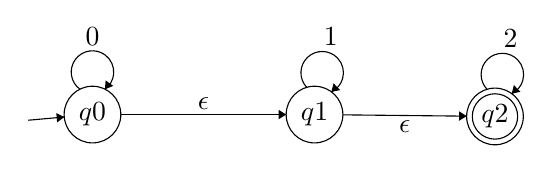
\begin{tikzpicture}[scale=0.12]
		\tikzstyle{every node}+=[inner sep=0pt]
		\draw [black] (63,-16.6) circle (3);
		\draw (63,-16.6) node {$q2$};
		\draw [black] (63,-16.6) circle (2.4);
		\draw [black] (20.4,-16.4) circle (3);
		\draw (20.4,-16.4) node {$q0$};
		\draw [black] (43.9,-16.4) circle (3);
		\draw (43.9,-16.4) node {$q1$};
		\draw [black] (62.163,-13.731) arc (223.99202:-64.00798:2.25);
		\draw (64.65,-9.36) node [above] {$2$};
		\fill [black] (64.77,-14.19) -- (65.69,-13.99) -- (65,-13.28);
		\draw [black] (19.077,-13.72) arc (234:-54:2.25);
		\draw (20.4,-9.15) node [above] {$0$};
		\fill [black] (21.72,-13.72) -- (22.6,-13.37) -- (21.79,-12.78);
		\draw [black] (13.6,-17) -- (17.41,-16.66);
		\fill [black] (17.41,-16.66) -- (16.57,-16.24) -- (16.66,-17.23);
		\draw [black] (43.082,-13.526) arc (223.6158:-64.3842:2.25);
		\draw (45.62,-9.17) node [above] {$1$};
		\fill [black] (45.68,-14) -- (46.61,-13.81) -- (45.92,-13.09);
		\draw [black] (23.4,-16.4) -- (40.9,-16.4);
		\fill [black] (40.9,-16.4) -- (40.1,-15.9) -- (40.1,-16.9);
		\draw (32.15,-15.9) node [above] {$\epsilon$};
		\draw [black] (46.9,-16.43) -- (60,-16.57);
		\fill [black] (60,-16.57) -- (59.21,-16.06) -- (59.19,-17.06);
		\draw (53.45,-17.01) node [below] {$\epsilon$};
	\end{tikzpicture}
	\caption{Transition diagram}
\end{figure}
\begin{eqnarray*}
	\epsilon-closure(q_0)&=& \{q_0,q_1,q_2\}\\
	\epsilon-closure(q_1)&=& \{q_1,q_2\}\\
	\epsilon-closure(q_2)&=& \{q_2\}\\
\end{eqnarray*}
\end{frame}
\begin{frame}{NFA with $\epsilon$ transitions($\epsilon$-NFA)}
	\textbf{Extended transition function($\hat{\delta}$) in $\epsilon$-NFA}
	\begin{enumerate}
		\item $\hat{\delta}(q,\epsilon)=\epsilon-closure(q)$
		\item for w in $\Sigma^*$ and a in $\Sigma$
		\begin{eqnarray*}
			\hat{\delta}(q,wa)&=&\epsilon-closure(p)\\
			&=&\{p/for\ some\ r\ in\ \hat{\delta}(q,w),p\ is\ in \ \delta(r,a)\}
		\end{eqnarray*}
	\item $\delta(R,a)=\bigcup\limits_{q\ in \ R}\delta(q,a)$
	\item $\hat{\delta}(R,w)=\bigcup\limits_{q\ in \ R}\hat{\delta}(q,w)$	
	\item $\hat{\delta}(q,a)=\epsilon-closure(\delta(\hat{\delta}(q,\epsilon),a))$
	\end{enumerate}
\end{frame}
\subsection{Equivalence of NFA with and without epsilon transitions}



\begin{frame}{Equivalence of NFA with and without epsilon transitions}
	\textbf{Conversion of Epsilon-NFA to NFA}
	\begin{enumerate}
		\item Find out all the $\epsilon$-transitions from each state from Q. That will be called as $\epsilon-closure(q_i)$ where, $qi \in Q$.
		\item Then, $\delta_1$ transitions can be obtained. The $\delta_1$ transitions means an $\epsilon$-closure on $\delta$ moves.
		\item Step 2 is repeated for each input symbol and for each state of given
		 NFA.
		\item By using the resultant status, the transition table for equivalent NFA without $\epsilon$ can be built.
	\end{enumerate}
\end{frame}
\begin{frame}{Equivalence of NFA with and without epsilon transitions}
	\textbf{Conversion of Epsilon-NFA to NFA}
	\begin{enumerate}
		\item Find out all the $\epsilon$-transitions from each state from Q. That will be called as $\epsilon-closure(q_i)$ where, $q_i$ $\in$Q.
		\item Then, $\delta_1$ transitions can be obtained. The $\delta_1$ transitions means an $\epsilon$-closure on $\delta$ moves.
		\item Step 2 is repeated for each input symbol and for each state of given NFA.
		\item By using the resultant status, the transition table for equivalent NFA without $\epsilon$ can be built.
	\end{enumerate}
\end{frame}
\begin{frame}{Equivalence of NFA with and without epsilon transitions}
	\textbf{Example:}Convert the given NFA with epsilon to NFA without epsilon.
	\begin{figure}
		\begin{center}
			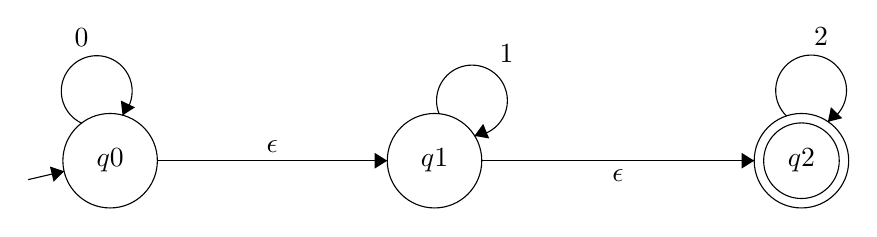
\begin{tikzpicture}[scale=0.2]
				\tikzstyle{every node}+=[inner sep=0pt]
				\draw [black] (18.2,-19.3) circle (3);
				\draw (18.2,-19.3) node {$q0$};
				\draw [black] (38.8,-19.3) circle (3);
				\draw (38.8,-19.3) node {$q1$};
				\draw [black] (62.1,-19.3) circle (3);
				\draw (62.1,-19.3) node {$q2$};
				\draw [black] (62.1,-19.3) circle (2.4);
				\draw [black] (21.2,-19.3) -- (35.8,-19.3);
				\fill [black] (35.8,-19.3) -- (35,-18.8) -- (35,-19.8);
				\draw (28.5,-18.8) node [above] {$\epsilon$};
				\draw [black] (39.094,-16.326) arc (202.08593:-85.91407:2.25);
				\draw (43.37,-13.07) node [above] {$1$};
				\fill [black] (41.34,-17.72) -- (42.27,-17.89) -- (41.89,-16.96);
				\draw [black] (13,-20.5) -- (15.28,-19.97);
				\fill [black] (15.28,-19.97) -- (14.38,-19.67) -- (14.61,-20.64);
				\draw [black] (41.8,-19.3) -- (59.1,-19.3);
				\fill [black] (59.1,-19.3) -- (58.3,-18.8) -- (58.3,-19.8);
				\draw (50.45,-19.8) node [below] {$\epsilon$};
				\draw [black] (61.156,-16.465) arc (226.14669:-61.85331:2.25);
				\draw (63.35,-12.02) node [above] {$2$};
				\fill [black] (63.78,-16.83) -- (64.69,-16.6) -- (63.97,-15.9);
				\draw [black] (16.395,-16.918) arc (244.88553:-43.11447:2.25);
				\draw (16.39,-12.08) node [above] {$0$};
				\fill [black] (18.99,-16.42) -- (19.78,-15.91) -- (18.88,-15.48);
			\end{tikzpicture}
		\end{center}
		\caption{NFA-With $\epsilon$ transition}
	\end{figure}
\end{frame}
\begin{frame}{Equivalence of NFA with and without epsilon transitions}
	\textbf{Solution:}We will first obtain $\epsilon-closure$ of each state
	\begin{eqnarray*}
		\epsilon-closure(q0) &=& \{q0,q1,q2\}\\
		\epsilon-closure(q1) &=&\{q1,q2\}\\
		\epsilon-closure(q2) &=& \{q2\}
	\end{eqnarray*}
	Now we will obtain $\delta$1 transitions for each state on each input symbol
		\begin{eqnarray*}
		\delta'(q0, 0) &=& \epsilon-closure(\delta(\hat{\delta}(q0, \epsilon),0))\\
		&=& \epsilon-closure(\delta(\epsilon-closure(q0),0))\\
		&=& \epsilon-closure(\delta(q0,q1,q2), 0))\\
		&=& \epsilon-closure(\delta(q0, 0) \cup \delta(q1, 0) \cup \delta(q2, 0) )\\
		&=& \epsilon-closure(q0 \cup \phi \cup \phi)\\
		&=& \epsilon-closure(q0)\\
		&=& \{q0,q1,q2\}
	\end{eqnarray*}
\end{frame}
\begin{frame}{Equivalence of NFA with and without epsilon transitions}
	\textbf{Solution cont..}
	\begin{eqnarray*}
		\delta'(q0,1) &=& \epsilon-closure(\delta(\hat{\delta}(q0,\epsilon),1))\\
		&=& \epsilon-closure(\delta(q0,q1,q2),1))\\
		&=& \epsilon-closure(\delta(q0, 1) \cup  \delta(q1, 1) \cup \delta(q2, 1) )\\
		&=& \epsilon-closure(\phi \cup q1 \cup \phi)\\
		&=& \epsilon-closure(q1)\\
		&=& \{q1, q2\}\\
		\delta'(q0, 2) &=& \epsilon-closure(\delta(\hat{\delta}(q0, \epsilon),2))\\
		&=& \epsilon-closure(\delta(q0,q1,q2), 2))\\
		&=& \epsilon-closure(\delta(q0, 2) \cup  \delta(q1, 2) \cup \delta(q2, 2) )\\
		&=& \epsilon-closure(\phi \cup \phi\cup q2)\\
		&=& \epsilon-closure(q2)\\
		&=& \{q2\}
	\end{eqnarray*}
\end{frame}
\begin{frame}{Equivalence of NFA with and without epsilon transitions}
	\textbf{Solution cont..}
	\begin{eqnarray*}
	\delta'(q1, 0) &=& \epsilon-closure(\delta(\hat{\delta}(q1, \epsilon),0))\\
		&=& \epsilon-closure(\delta(q1,q2), 0))\\
		&=& \epsilon-closure(\delta(q1, 0) \cup \delta(q2, 0) )\\
		&=& \epsilon-closure(\phi \cup \phi)\\
		&=& \epsilon-closure(\phi)\\
		&=& \phi\\
		\delta'(q1,1) &=& \epsilon-closure(\delta(\hat{\delta}(q1, \epsilon),1))\\
		&=& \epsilon-closure(\delta(q1,q2), 1))\\
		&=& \epsilon-closure(\delta(q1, 1) \cup \delta(q2, 1) )\\
		&=& \epsilon-closure(q1 \cup \phi)\\
		&=& \epsilon-closure(q1)\\
		&=& \{q1,q2\}
	\end{eqnarray*}
\end{frame}
\begin{frame}{Equivalence of NFA with and without epsilon transitions}
	\textbf{Solution cont..}
	\begin{eqnarray*}
	\delta'(q1, 2) &=& \epsilon-closure(\delta(\hat{\delta}(q1, \epsilon),2))\\
	&=& \epsilon-closure(\delta(q1,q2), 2))\\
	&=& \epsilon-closure(\delta(q1, 2) \cup \delta(q2, 2) )\\
	&=& \epsilon-closure(\phi \cup q2)\\
	&=& \epsilon-closure(q2)\\
	&=& \{q2\}\\
	\delta'(q2, 0) &=& \epsilon-closure(\delta(\hat{\delta}(q2, \epsilon),0))\\
	&=& \epsilon-closure(\delta(q2), 0))\\
	&=& \epsilon-closure(\delta(q2, 0))\\
	&=& \epsilon-closure(\phi)\\
	&=& \phi\\
	\end{eqnarray*}
\end{frame}
\begin{frame}{Equivalence of NFA with and without epsilon transitions}
	\textbf{Solution cont..}
	\begin{eqnarray*}
		\delta'(q2, 1) &=& \epsilon-closure(\delta(\hat{\delta}(q2, \epsilon),1))\\
		&=& \epsilon-closure(\delta(q2), 1)\\
		&=& \epsilon-closure(\delta(q2, 1))\\
		&=& \epsilon-closure(\phi)\\
		&=& \phi\\
		\delta'(q2, 2) &=& \epsilon-closure(\delta(\hat{\delta}(q2, \epsilon),))\\
		&=& \epsilon-closure(\delta(q2), 2))\\
		&=& \epsilon-closure(\delta(q2, 2))\\
		&=& \epsilon-closure(q2)\\
		&=& \{q2\}
	\end{eqnarray*}
\end{frame}
\begin{frame}{Equivalence of NFA with and without epsilon transitions}
	\textbf{Solution cont..}\\Now, we will summarize all the computed $\delta$' transitions as given below
	\begin{eqnarray*}
		\delta'(q0,0)&=&\{q0,q1,q2\}\\
		\delta'(q0,1)&=&\{q1,q2\}\\
		\delta'(q0,2)&=&\{q2\}\\
		\delta'(q1,0)&=&\{ \phi \}\\
		\delta'(q1,1)&=&\{q1,q2\}\\
		\delta'(q1,2)&=&\{q2\}\\
		\delta'(q2,0)&=&\{ \phi \}\\
		\delta'(q2,1)&=&\{ \phi \}\\
		\delta'(q2,2)&=&\{q2\}\\
	\end{eqnarray*}
\end{frame}
\begin{frame}{Equivalence of NFA with and without epsilon transitions}
	\textbf{Solution cont..}
	The transition table is given below
	\begin{table}
		\begin{tabular}{c||c|c|c}
			$\delta$&	0&	1&	2\\
			\hline
			\hline
			$\rightarrow$*q0&	\{q0,q1,q2\}&	\{q1,q2\}&	\{q2\}\\
			\hline
			q1& $\phi$&	\{q1,q2\}&	\{q2\}\\
			\hline
			*q2&	$\phi$&	$\phi$&	\{q2\}
		\end{tabular}
	\caption{Transition table NFA without $\epsilon$ transition}
	\end{table}
\begin{figure}
	\begin{center}
		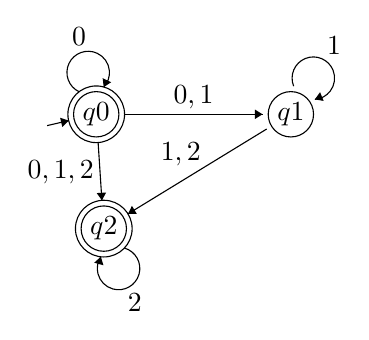
\begin{tikzpicture}[scale=0.12]
			\tikzstyle{every node}+=[inner sep=0pt]
			\draw [black] (18.2,-19.3) circle (3);
			\draw (18.2,-19.3) node {$q0$};
			\draw [black] (18.2,-19.3) circle (2.4);
			%\draw [black] (38.8,-19.3) circle (3);
			\draw (38.8,-19.3) node {$q1$};
			\draw [black] (38.8,-19.3) circle (2.4);
			\draw [black] (19,-31.4) circle (3);
			\draw (19,-31.4) node {$q2$};
			\draw [black] (19,-31.4) circle (2.4);
			\draw [black] (21.2,-19.3) -- (35.8,-19.3);
			\fill [black] (35.8,-19.3) -- (35,-18.8) -- (35,-19.8);
			\draw (28.5,-18.8) node [above] {$0,1$};
			\draw [black] (39.094,-16.326) arc (202.08593:-85.91407:2.25);
			\draw (43.37,-13.07) node [above] {$1$};
			\fill [black] (41.34,-17.72) -- (42.27,-17.89) -- (41.89,-16.96);
			\draw [black] (13,-20.5) -- (15.28,-19.97);
			\fill [black] (15.28,-19.97) -- (14.38,-19.67) -- (14.61,-20.64);
			\draw [black] (16.395,-16.918) arc (244.88553:-43.11447:2.25);
			\draw (16.39,-12.08) node [above] {$0$};
			\fill [black] (18.99,-16.42) -- (19.78,-15.91) -- (18.88,-15.48);
			\draw [black] (18.4,-22.29) -- (18.8,-28.41);
			\fill [black] (18.8,-28.41) -- (19.25,-27.58) -- (18.25,-27.64);
			\draw (18,-25.39) node [left] {$0,1,2$};
			\draw [black] (21.171,-33.454) arc (74.32314:-213.67686:2.25);
			\draw (22.28,-38.25) node [below] {$2$};
			\fill [black] (18.69,-34.37) -- (17.99,-35.01) -- (18.96,-35.28);
			\draw [black] (36.24,-20.86) -- (21.56,-29.84);
			\fill [black] (21.56,-29.84) -- (22.5,-29.85) -- (21.98,-28.99);
			\draw (27.15,-24.85) node [above] {$1,2$};
		\end{tikzpicture}
	\end{center}
\caption{Transition digram NFA without $\epsilon$ transition}
\end{figure}
\end{frame}
\begin{frame}{Conversion NFA with epsilon to DFA }
	The method for converting the NFA with $\epsilon$ to DFA is explained below
	\begin{itemize}
		\item Consider $M=(Q, \Sigma, \delta ,q0,F)$ is NFA with $\epsilon$.
		\item  We have to convert this NFA with $\epsilon$ to equivalent DFA denoted by $M_D=(Q_D,\Sigma, \delta_D,q0,F_D)$
		 
			\item Then obtain, $\epsilon-closure(q0) =\{p1,p2,p3,……pn\}$
			\item then $[p1,p2,p2,….pn]$ becomes a start state of DFA
			\item now$[p1,p2,p3,….pn] \in Q_D$
		
		\item We will obtain $\delta$ transition on [p1,p2,p3,…pn] for each input.
		
		\begin{itemize}
			 \item $\delta_D([p1,p2,p3,..pn],a) = \epsilon -closure(\delta(p1,a)$
		 $\cup\  \delta(p2,a2)\cup……………… \delta(pn,a))$
			
			\item $= \bigcup\limits_{i=1}^{n}  \epsilon-closure d(pi,a)$
			
			Where a is input $\in \Sigma$
		\end{itemize}
	\item The state obtained $[p1,p2,p3,…pn] \in Q_D$ .
	
	\item The states containing final state in pi is a final state in DFA
	\end{itemize}
\end{frame}
\begin{frame}{Conversion NFA with epsilon to DFA }
	\textbf{Example:}
	Convert the following NFA with epsilon to equivalent DFA
	\begin{figure}
		\begin{center}
			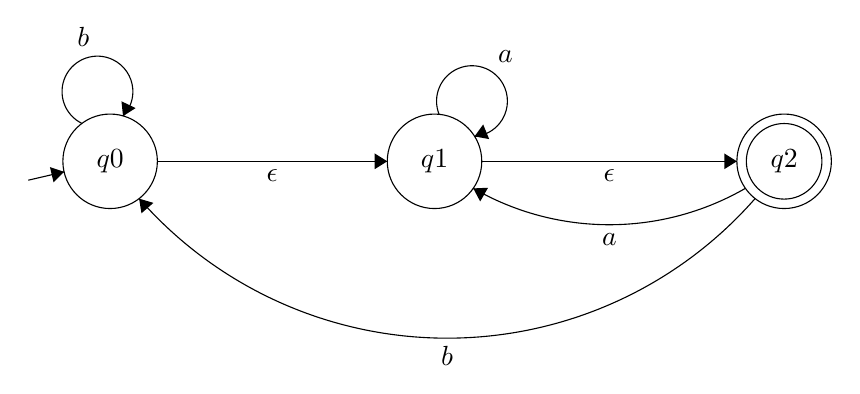
\begin{tikzpicture}[scale=0.2]
				\tikzstyle{every node}+=[inner sep=0pt]
				\draw [black] (18.2,-19.3) circle (3);
				\draw (18.2,-19.3) node {$q0$};
				\draw [black] (38.8,-19.3) circle (3);
				\draw (38.8,-19.3) node {$q1$};
				\draw [black] (61,-19.3) circle (3);
				\draw (61,-19.3) node {$q2$};
				\draw [black] (61,-19.3) circle (2.4);
				\draw [black] (21.2,-19.3) -- (35.8,-19.3);
				\fill [black] (35.8,-19.3) -- (35,-18.8) -- (35,-19.8);
				\draw (28.5,-19.8) node [below] {$\epsilon$};
				\draw [black] (39.094,-16.326) arc (202.08593:-85.91407:2.25);
				\draw (43.31,-13.07) node [above] {$a$};
				\fill [black] (41.34,-17.72) -- (42.27,-17.89) -- (41.89,-16.96);
				\draw [black] (13,-20.5) -- (15.28,-19.97);
				\fill [black] (15.28,-19.97) -- (14.38,-19.67) -- (14.61,-20.64);
				\draw [black] (16.42,-16.899) arc (244.2807:-43.7193:2.25);
				\draw (16.5,-12.07) node [above] {$b$};
				\fill [black] (19.02,-16.43) -- (19.82,-15.92) -- (18.92,-15.49);
				\draw [black] (41.8,-19.3) -- (58,-19.3);
				\fill [black] (58,-19.3) -- (57.2,-18.8) -- (57.2,-19.8);
				\draw (49.9,-19.8) node [below] {$\epsilon$};
				\draw [black] (58.543,-21.015) arc (-60.04117:-119.95883:17.308);
				\fill [black] (41.26,-21.02) -- (41.7,-21.85) -- (42.2,-20.98);
				\draw (49.9,-23.83) node [below] {$a$};
				\draw [black] (59.157,-21.665) arc (-41.22581:-138.77419:26.003);
				\fill [black] (20.04,-21.67) -- (20.19,-22.6) -- (20.95,-21.94);
				\draw (39.6,-31.03) node [below] {$b$};
			\end{tikzpicture}
		\end{center}
	\caption{NFA with $\epsilon$ transition}
	\end{figure}
\end{frame}
\begin{frame}{Conversion NFA with epsilon to DFA }
	\textbf{Solution:}\\To convert this NFA with epsilon, we will first find the $\epsilon$ -closures, 
	\begin{eqnarray*}
		\epsilon -closure(q0)&=&\{q0,q1,q2\}\\
		\epsilon -closure(q1)&=&\{q1,q2\}\\
		\epsilon -closure(q2)&=&\{q2\}
	\end{eqnarray*}
When, $\epsilon-closure(q0)=\{q0,q1,q2\}$, we will call this state as A.

\par Now, let us find transition on A with every input symbol
\begin{eqnarray*}
	\delta'(A, a) &=& \epsilon-closure(\delta(A,a))\\
	&=& \epsilon-closure(\delta(q0,q1,q2), a))\\
	&=& \epsilon-closure(\delta(q0, a) \cup  \delta(q1,a) \cup  \delta(q2,a) )\\
	&=& \epsilon-closure(\phi\cup q1 \cup q2)\\
	&=& \epsilon-closure(q1\cup q2)\\
	&=& \{q1, q2\} \ let \ us\  call\  it \ as \ state\  B\\
\end{eqnarray*}
	
\end{frame}
\begin{frame}{Conversion NFA with epsilon to DFA }
	\textbf{Solution cont..}
	\begin{eqnarray*}
		\delta'(A, b) &=& \epsilon-closure(\delta(A,b))\\
		&=& \epsilon-closure(\delta(q0,q1,q2), b))\\
		&=& \epsilon-closure(\delta(q0, b) \cup  \delta(q1,b) \cup \delta(q2,b) )\\
		&=& \epsilon-closure(q0 \cup \phi \cup q0)\\
		&=& \epsilon-closure(q0)\\
		&=& \{q0,q1, q2\}\  its \ nothing\  but\  state\  A\\
		\delta'(B, a) &=& \epsilon-closure(\delta(B,a))\\
		&=& \epsilon-closure(\delta(q1,q2), a))\\
		&=& \epsilon-closure(\delta(q1,a) \cup \delta(q2,a) )\\
		&=& \epsilon-closure(q1 \cup q2)\\
		&=& \epsilon-closure(q1)\\
		&=& \{q1, q2\} \ its\  nothing\  but\  state\  B\\
	\end{eqnarray*}
\end{frame}
\begin{frame}{Conversion NFA with epsilon to DFA }
	\textbf{Solution cont..}
	\begin{eqnarray*}
		\delta'(B, b) &=& \epsilon-closure(\delta(B,b))\\
		&=& \epsilon-closure(\delta(q1,q2), b))\\
		&=& \epsilon-closure(\delta(q1,b) \cup \delta(q2,b) )\\
		&=& \epsilon-closure(\phi \cup q0)\\
		&=& \epsilon-closure(q0)\\
		&=& \{q0,q1, q2\}\  its \ nothing\  but\  state\  A\\
	\end{eqnarray*}
\end{frame}
\begin{frame}{Conversion NFA with epsilon to DFA }
	\textbf{Solution cont..}
	Hence, the transition table for the generated DFA is as follows
	\begin{table}
		\begin{tabular}{c||c|c}
			$\delta$ &	a &	b \\
			\hline
			\hline
			$\rightarrow$*A&	B	&A \\
			\hline
		*B&	B&	A
		\end{tabular}
	\caption{DFA without $\epsilon$}
	\end{table}
\begin{figure}
	\begin{center}
		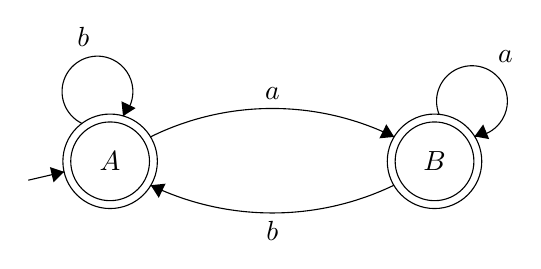
\begin{tikzpicture}[scale=0.2]
			\tikzstyle{every node}+=[inner sep=0pt]
			\draw [black] (18.2,-19.3) circle (3);
				\draw [black] (18.2,-19.3) circle (2.5);
			\draw  (18.2,-19.3) node {$A$};
			\draw [black] (38.8,-19.3) circle (3);
					\draw [black] (38.8,-19.3) circle (2.5);
			\draw (38.8,-19.3) node {$B$};
			\draw [black] (20.763,-17.749) arc (116.26382:63.73618:17.483);
			\fill [black] (36.24,-17.75) -- (35.74,-16.95) -- (35.3,-17.84);
			\draw (28.5,-15.44) node [above] {$a$};
			\draw [black] (39.094,-16.326) arc (202.08593:-85.91407:2.25);
			\draw (43.31,-13.07) node [above] {$a$};
			\fill [black] (41.34,-17.72) -- (42.27,-17.89) -- (41.89,-16.96);
			\draw [black] (13,-20.5) -- (15.28,-19.97);
			\fill [black] (15.28,-19.97) -- (14.38,-19.67) -- (14.61,-20.64);
			\draw [black] (16.42,-16.899) arc (244.2807:-43.7193:2.25);
			\draw (16.5,-12.07) node [above] {$b$};
			\fill [black] (19.02,-16.43) -- (19.82,-15.92) -- (18.92,-15.49);
			\draw [black] (36.219,-20.821) arc (-64.31186:-115.68814:17.806);
			\fill [black] (20.78,-20.82) -- (21.29,-21.62) -- (21.72,-20.72);
			\draw (28.5,-23.08) node [below] {$b$};
		\end{tikzpicture}
	\end{center}
\caption{DFA without $\epsilon$ diagram}
\end{figure}
\end{frame}
\begin{frame}{Equivalence of NFA with and without epsilon transitions}
\begin{block}{Theorem 1.1}
If L is a language accepted by NFA with $\epsilon$- transition, Then L is accepted by NFA without
$\epsilon$-transition.
\end{block}
\textbf{Proof:}
\begin{itemize}
	\item Let $M = (Q,\Sigma,\delta,q0,F)$ be a NFA with $\epsilon$- transition, then we need to construct an NFA,$M’ = (Q,\Sigma,\delta’,q_0,F’)$
	\item Where
	$$
	F'=\begin{cases}
		F \cup \{q_0\} & if \epsilon-closure(q_0)\  contains\  a \ state\  from\  F,  \\
		F & Otherwise
	\end{cases}
	$$
 and
	$$\delta'(q,a)=\delta(q,a) for\  q\in Q\  and\ a \in \Sigma  $$
\end{itemize}
\end{frame}
\begin{frame}{Equivalence of NFA with and without epsilon transitions}
	\textbf{Proof Cont..}\\
	\textbf{Basis}
	\begin{itemize}
		\item $|x|=1$ then x is a symbol a and
		$$\delta'(q0,a)=\delta(q0,a)\ by \ definition \ of\ \delta'$$
	\end{itemize}
	\textbf{Induction}
\begin{itemize}
\item Assume the hypothysis is true for the string of length m or less
$$i.e\  \ \ \hat{\delta}'(q0,x)=\hat{\delta}(q0,x)$$
\end{itemize}
To prove this theorem we must show that 
$$\hat{\delta}'(q0,xa)=\hat{\delta}(q0,xa)\  \ where\  |xa|=m+1$$
\end{frame}
\begin{frame}{Equivalence of NFA with and without epsilon transitions}
	\small
	\begin{eqnarray*}
\hat{\delta}(q0,xa) &=& \delta'(\hat{\delta}'(q0,x),a)\\
					&=& \delta'(\hat{\delta}(q0,x),a) \ \ by\ hypothysis\\				
	\end{eqnarray*}
let $\hat{\delta}(q0,x)=P=\{q0,q1,q2,q3,......q_n\}$

\begin{eqnarray*}
	therefor\ \hat{\delta}'(q0,xa)&=&\delta'(P,a)\\
							&=&\bigcup\limits_{q \in P}	\delta'(q,a)\\
							&=&\bigcup\limits_{q \in P}	\delta(q,a)\\
							&=&	\delta(P,a)\\
							&=&	\delta(\hat{\delta}(q0,x),a)\\
							&=&	\hat{\delta}
							(q0,xa)\\	
						Thus\  \delta'(q0,xa)=\hat{\delta}(q0,xa)
\end{eqnarray*}
\end{frame}
\section{Regular Grammar}
\begin{frame}{Regular Grammar}
	\textbf{Chomsky Hierarchy in Theory of Computation}
	\begin{figure}
		\includegraphics[scale=.6]{img1/m2}
		\caption{Chomsky Hierarchy in Theory of Computation}
	\end{figure}
\end{frame}
\begin{frame}{Regular Grammar}
	\textbf{Regular Grammar(RG)-Type 3}
	\begin{itemize}
		\item Regular grammar generates regular language. 
		\item Regular Languages are recognized by using finite state automata.
	\end{itemize}

\end{frame}
\begin{frame}{Regular Grammar}
	\textbf{Formal definition of Regular Grammar(RG)-Type 3}
	\begin{itemize}
		\item A Regular Grammar ‘G’ can be formally described using four tuples as $G = (V, T, P, S)$
		\item where,
		\begin{itemize}
			\item V = Set of Variables or Non-Terminal Symbols(Capital letters)
			\item T = Set of Terminal Symbols(Small letters, Numbers etc)
			\item S = Start Symbol $S\in V$
			\item P = Production Rules for Terminals and Non-Terminals

		\end{itemize}
	\end{itemize}
		\begin{equation*}
		\begin{split}\begin{array}{c}
				\mbox{All productions are of the form} \\
				A \rightarrow xB \\
				A \rightarrow Cx \\
				A \rightarrow x \\
				\mbox{where}\ A,B,C \in V, x \in T^*
		\end{array}\end{split}
	\end{equation*}
\end{frame}
\begin{frame}{Regular Grammar}
	\textbf{Types of regular grammar:}
	\begin{enumerate}
		\item Right linear grammar(RLG)
		\item Left Linear grammar(LLG)
	\end{enumerate}
\end{frame}

\begin{frame}{Regular Grammar}
	\textbf{Right-linear grammar}
	\begin{itemize}
		\item A grammar is said to be Right-linear if all productions are of the form:
	\end{itemize}
	\begin{equation*}
		\begin{split}\begin{array}{c}
				A \rightarrow xB \\
				A \rightarrow xC \\
				A \rightarrow y \\
				\mbox{where}\ A,B,C \in V, x,y \in T^*
		\end{array}\end{split}
	\end{equation*}
	\textbf{Example}\\
	\begin{eqnarray*}
				G &=& (\{S,B\},\{a,b\},P,S),\\
				P &=& \\
				&&S \rightarrow aB | bS | \epsilon \\
				&&B \rightarrow aS | bB \\
		\end{eqnarray*}

\end{frame}
\begin{frame}{Regular Grammar}
	\textbf{Left Linear grammar}
	\begin{itemize}
		\item A grammar is said to be Left Linear if all productions are of the form:
	\end{itemize}
	\begin{equation*}
		                                       \begin{split}\begin{array}{c}
				A \rightarrow Bx \\
				A \rightarrow Cy \\
				A \rightarrow x \\
				\mbox{where}\ A,B,C \in V, x,y \in T^*
		\end{array}\end{split}
	\end{equation*}
\textbf{Example}\\
\begin{eqnarray*}
	G &=& (\{S,B\},\{a,b\},P,S),\\
	P &=& \\
	&&S \rightarrow Ba | Sb | \epsilon
	 \\
	&&B \rightarrow Sa | Bb \\
\end{eqnarray*}
\end{frame}
\begin{frame}{Regular Grammar}
	\textbf{Derivation of sentences}
	\\ \textbf{Grammar}
	\begin{eqnarray*}
	A &\rightarrow& aB\\
	B &\rightarrow& aB\\
	B &\rightarrow& bB\\
	B&\rightarrow& \epsilon
	\end{eqnarray*}
	\\ \textbf{Derivation from the above grammar}
\begin{eqnarray*}
	A &\implies& aB \implies a\\
	A &\implies& aB \implies aaB \implies aa\\
	A &\implies& aB \implies abB \implies ab\\
	A &\implies& aB \implies aaB \implies aaaB \implies aaa
\end{eqnarray*}
Language generated by the grammar is $L(G)=\{ax|x\in \{a,b\}^*\}$
\end{frame}
\begin{frame}{Regular Grammar}
\begin{itemize}
	\item Language generated by the grammar is $L(G)=\{ax|x\in \{a,b\}^*\}$
	\item i.e $a(a+b)^*$(Called Regular Expression)
\end{itemize}
	
\end{frame}

\begin{frame}{Regular Grammar}
	\textbf{Language generated by Regular Grammar}
	\begin{itemize}
		\item The class of languages generated by the family of regular grammar is precisely the set of Regular Language
		\begin{itemize}
			\item The language genereated by a Regular grammar is Regular
			\item Any Regular Language can be generated by a Regular Grammar
		\end{itemize}
	\end{itemize}
\end{frame}
\begin{frame}{Regular Grammar}
	\textbf{Converting	Regular	Grammar	to	DFA}\\
	Assume	that	a	regular	grammar	is	given	in	its	right-linear	form,	this	grammar	may	be	easily	converted	to	
	a	DFA.		A	right-linear	grammar,	defined	by	$G	=	(V,	T,	S,	P),$	may	be	converted	to	a	DFA,	defined	by	$M	=	(Q,	
	\Sigma,	\delta,	q0, F)$	by:
	\begin{itemize}
		\item[1] Create	a	state	for	each	variable.
		\item[2] Convert	each	production	rule	into	a	transition.
		\begin{itemize}
			\item[a] If	the	production	rule	is	of	the	form	$V_i\rightarrow aV_j$,	where	$a \in T$, add	the	transition	$\delta(V_i,a)	=	V_j$
			to	M.		For	example,	$V_0 \rightarrow aV_1$ becomes: 
			\begin{center}
				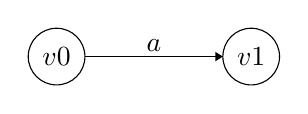
\begin{tikzpicture}[scale=0.12]
					\tikzstyle{every node}+=[inner sep=0pt]
					\draw [black] (18.2,-19.3) circle (3);
					\draw (18.2,-19.3) node {$v0$};
					\draw [black] (38.8,-19.3) circle (3);
					\draw (38.8,-19.3) node {$v1$};
					\draw [black] (21.2,-19.3) -- (35.8,-19.3);
					\fill [black] (35.8,-19.3) -- (35,-18.8) -- (35,-19.8);
					\draw (28.5,-18.8) node [above] {$a$};
				\end{tikzpicture}
			\end{center}
		\end{itemize}
	\end{itemize}
\end{frame}
\begin{frame}{Regular Grammar}
	\begin{itemize}
		\item[b]If	the	production	rule	is	of	the form	$V_i \rightarrow wV_j,$	where	$w	\in T^*$, create	a	series	of	states	
		which	derive	w	and	end	in	$V_j$.			Add	the	states	in	between	to	Q.		For	example,	$V_0 \rightarrow abcV_1$ becomes
		\begin{center}
			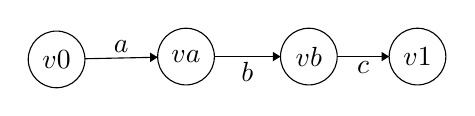
\begin{tikzpicture}[scale=0.12]
				\tikzstyle{every node}+=[inner sep=0pt]
				\draw [black] (18.2,-19.3) circle (3);
				\draw (18.2,-19.3) node {$v0$};
				\draw [black] (31.9,-19) circle (3);
				\draw (31.9,-19) node {$va$};
				\draw [black] (44.9,-19) circle (3);
				\draw (44.9,-19) node {$vb$};
				\draw [black] (56.4,-19) circle (3);
				\draw (56.4,-19) node {$v1$};
				\draw [black] (21.2,-19.23) -- (28.9,-19.07);
				\fill [black] (28.9,-19.07) -- (28.09,-18.58) -- (28.11,-19.58);
				\draw (25.04,-18.63) node [above] {$a$};
				\draw [black] (34.9,-19) -- (41.9,-19);
				\fill [black] (41.9,-19) -- (41.1,-18.5) -- (41.1,-19.5);
				\draw (38.4,-19.5) node [below] {$b$};
				\draw [black] (47.9,-19) -- (53.4,-19);
				\fill [black] (53.4,-19) -- (52.6,-18.5) -- (52.6,-19.5);
				\draw (50.65,-19.5) node [below] {$c$};
			\end{tikzpicture}
		\end{center}
	\item[c] If	the	production	rule	is	of	the	form	$V_i \rightarrow w$,	where	$w	\in T^*$, create	a	series	of	states	
	which	derive	w and	end	in	a	final	state.		For	example,	$V_0 \rightarrow a$	becomes:
\begin{center}
	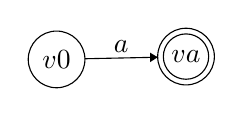
\begin{tikzpicture}[scale=0.12]
		\tikzstyle{every node}+=[inner sep=0pt]
		\draw [black] (18.2,-19.3) circle (3);
		\draw (18.2,-19.3) node {$v0$};
		\draw [black] (31.9,-19) circle (3);
		\draw (31.9,-19) node {$va$};
		\draw [black] (31.9,-19) circle (2.4);
		\draw [black] (21.2,-19.23) -- (28.9,-19.07);
		\fill [black] (28.9,-19.07) -- (28.09,-18.58) -- (28.11,-19.58);
		\draw (25.04,-18.63) node [above] {$a$};
	\end{tikzpicture}
\end{center}
	\end{itemize}
\end{frame}
\begin{frame}{Regular Grammar}
\begin{block}{Theorem}
Let G=(V,T,P,S) be a right linear grammar. then L(G) is regular language
\end{block}
\proofname \\
We assume that $V =\{V_0, V_1, ...\},\  that\  S = V_0,$ and that we have
productions of the form $V_0 \rightarrow v_1V_i, V_i \rightarrow v_2V_j, ...\  or\  V_n\rightarrow v_l, ....$ If w is a
string in L(G), then because of the form of the productions
\small
\begin{eqnarray*}
	V_0 &\implies& v_1V_i\\
	&\implies& v_1v_2V_j\\
	&.&\\
	&.&\\
	&.&\\
	&\implies& v_1v_2…v_kV_n\\
	&\implies& v_1v_2…v_kv_l = w.
\\
\end{eqnarray*}
\end{frame}
\begin{frame}{Regular Grammar}
	The automaton to be constructed will reproduce the derivation by
	consuming each of these v’s in turn. The initial state of the automaton will be labeled $V_0$
	, and for each variable $V_i$
	there will be a nonfinal state
	labeled $V_i$
	. For each production
	$$V_i \implies a_1a_2..... a_mV_j,$$
	the automaton will have transitions to connect $V_i$ and $V_j$
	that is, $\delta$ will be
	defined so that
	$$\delta^* (V_i, a_1a_2.... a_m) = V_j$$
	For each production
	$$V_i \implies a_1a_2.... a_m,$$
	the corresponding transition of the automaton will be
	$$\delta^* (V_i, a_1a_2.... a_m) = V_f
	,$$
\end{frame}	
\begin{frame}{Regular Grammar}
	where $V_f$
	is a final state. The intermediate states that are needed to do
	this are of no concern and can be given arbitrary labels.
	\begin{figure}
		\includegraphics[scale=.5]{img1/m3}
		%\caption{Chomsky Hierarchy in Theory of Computation}
	\end{figure}

\end{frame}	
\begin{frame}{Regular Grammar}
Suppose now that $w \in L(G)$ so that the above equation is satisfied. In the nfa there
is, by construction, a path from $V_0$
to $V_i$
labeled v1
, a path from $V_i$
to $V_j$
labeled $v_2$
, and so on, so that clearly

$$V_f \in \delta^* (V_0, w),$$
and w is accepted by M.
\par Conversely, assume that w is accepted by M. Because of the way in
which M was constructed, to accept w the automaton has to pass through
a sequence of states $V_0$
, $V_i$
, ....to $V_f$
, using paths labeled $v_1$
, $v_2$
, ....
Therefore, w must have the form
$$w = v_1v_2 ··· v_kv_l$$
and the derivation
$$V_o \implies v_1V_i \implies v_1v_2V_j
\xRightarrow{*} v_1v_2…v_kV_k \implies v_1v_2…v_kv_1$$
is possible. Hence w is in L (G), and the theorem is proved.
\end{frame}		
\begin{frame}{Regular Grammar}
\begin{block}{Theorem}
	If L is a regular language on the alphabet $\Sigma$, then there exists a right-linear
grammar $G = (V, \Sigma, S, P)$ such that $L = L (G)$.

\end{block}
	\proofname \\
	Let $M = (Q, \Sigma, \delta, q_0
	, F)$ be a dfa that accepts L. We assume that$ Q = \{q_0	, q_1,..., q_n\} and \Sigma = \{a_1, a_2,...., a_m\}$. Construct the right-linear grammar $G = (V, \Sigma, S, P)$ with $V = \{q_0, q_1	,..., q_n\}$

	and $S = q_0$. For each transition $\delta(q_i, a_j	) = q_k$
	of M, we put in P the production
	$$q_i \rightarrow a_jq_k.$$
	In addition, if $q_k$
	is in F, we add to P the production
	$$q_k \rightarrow \lambda.$$
	
\end{frame}			
\begin{frame}{Regular Grammar}
	\proofname cont.. \\
	\small
	We first show that G defined in this way can generate every string in L.
	Consider $w \in L$ of the form $w = a_ia_j... a_ka_l$
	For M to accept this string it must make moves via
	\begin{eqnarray*}
		\delta(q_0,a_i) &=& q_p,\\
		\delta(q_p,a_j) &=& q_r,\\
			&.&\\
		&.&\\
			\delta(q_s,a_k)&=& q_t,\\
			\delta_(q_t,a_l)&=&q_f \in F.\\
	\end{eqnarray*}
\end{frame}	
\begin{frame}{Regular Grammar}
	\proofname cont.. \\
	By construction, the grammar will have one production for each of these $\delta$’s.
	Therefore, we can make the derivation

	\begin{eqnarray*}
		q_0 &\implies& a_iq_p \implies a_ia_jq_r \xRightarrow{*} a_ia_j… a_kq_t\\
		&\implies& a_ia_j… a_ka_lq_f \implies a_ia_j… a_ka_l,
	\end{eqnarray*}
with the grammar G, and $w \in L(G)$.
\par Conversely, if$ w \in L(G)$, then its derivation must have the form the above equation. But this
implies that $\delta^* (q_0, a_ia_j...a_ka_l) = q_f$, completing the proof.
\end{frame}		
\end{document}